% !TeX spellcheck = hu_HU
% !TeX encoding = UTF-8
% !TeX program = xelatex
% TODO Change language to en_GB (recommended) or en_US for English documents
\documentclass[11pt,a4paper,oneside]{report}             % Single-side
%\documentclass[11pt,a4paper,twoside,openright]{report}  % Duplex

% thanks to http://tex.stackexchange.com/a/47579/71109
\usepackage{ifxetex}
\usepackage{ifluatex}
\newif\ifxetexorluatex % a new conditional starts as false
\ifnum 0\ifxetex 1\fi\ifluatex 1\fi>0
   \xetexorluatextrue
\fi

\ifxetexorluatex
  \usepackage{fontspec}
\else
  \usepackage[T1]{fontenc}
  % Not needed with LaTeX 2018 or later
  \usepackage[utf8]{inputenc}
  \usepackage[lighttt]{lmodern}
\fi

\usepackage[english,magyar]{babel} % Alapértelmezés szerint utoljára definiált nyelv lesz aktív, de később külön beállítjuk az aktív nyelvet.

%\usepackage{cmap}
\usepackage{amsfonts,amsmath,amssymb} % Mathematical symbols.
%\usepackage[ruled,boxed,resetcount,linesnumbered]{algorithm2e} % For pseudocodes. % beware: this is not compatible with LuaLaTeX, see http://tex.stackexchange.com/questions/34814/lualatex-and-algorithm2e
\usepackage{booktabs} % For publication quality tables for LaTeX
\usepackage{graphicx}

%\usepackage{fancyhdr}
%\usepackage{lastpage}

\usepackage{anysize}
%\usepackage{sectsty}
\usepackage{setspace} % For setting line spacing

\usepackage[unicode]{hyperref} % For hyperlinks in the generated document.
\usepackage{xcolor}
\usepackage{listings} % For source code snippets.

\usepackage[amsmath,thmmarks]{ntheorem} % Theorem-like environments.

\usepackage[hang]{caption}

\singlespacing

\newcommand{\selecthungarian}{
	\selectlanguage{magyar}
	\setlength{\parindent}{2em}
	\setlength{\parskip}{0em}
	\frenchspacing
}

\newcommand{\selectenglish}{
	\selectlanguage{english}
	\setlength{\parindent}{0em}
	\setlength{\parskip}{0.5em}
	\nonfrenchspacing
	\renewcommand{\figureautorefname}{Figure}
	\renewcommand{\tableautorefname}{Table}
	\renewcommand{\partautorefname}{Part}
	\renewcommand{\chapterautorefname}{Chapter}
	\renewcommand{\sectionautorefname}{Section}
	\renewcommand{\subsectionautorefname}{Section}
	\renewcommand{\subsubsectionautorefname}{Section}
}

\usepackage[numbers]{natbib}
\usepackage{xspace}

\usepackage{pdfpages} % For insert PDF file as is 

%TODO Set the main variables
\newcommand{\vikszerzoVezeteknev}{Csepi}
\newcommand{\vikszerzoKeresztnev}{Árpád}

\newcommand{\vikkonzulensAMegszolitas}{dr.~}
\newcommand{\vikkonzulensAVezeteknev}{Farkas}
\newcommand{\vikkonzulensAKeresztnev}{Károly}

\newcommand{\vikkonzulensBMegszolitas}{}
\newcommand{\vikkonzulensBVezeteknev}{Gyurácz}
\newcommand{\vikkonzulensBKeresztnev}{Kristóf}

\newcommand{\vikkonzulensCMegszolitas}{}
\newcommand{\vikkonzulensCVezeteknev}{}
\newcommand{\vikkonzulensCKeresztnev}{}

\newcommand{\vikcim}{Istio operator CLI fejlesztése} % Cím
\newcommand{\viktanszek}{\hit} % Tanszék
\newcommand{\vikdoktipus}{\bsc} % Dokumentum típusa (\bsc vagy \msc)
\newcommand{\vikmunkatipusat}{szakdolgozatot} % a "hallgató nyilatkozat" részhez: szakdolgozatot vagy diplomatervet

%--------------------------------------------------------------------------------------
% TDK-specifikus változók
%--------------------------------------------------------------------------------------
\newcommand{\tdkszerzoB}{Második Szerző} % Második szerző neve; hagyd üresen, ha egyedül írtad a TDK-t.
\newcommand{\tdkev}{2014} % A dolgozat írásának éve (pl. "2014") (Ez OTDK-nál eltérhet az aktuális évtől.)

% További adatok az OTDK címlaphoz (BME-s TDK-hoz nem kell kitölteni)
\newcommand{\tdkevfolyamA}{IV} % Első szerző évfolyama, római számmal (pl. IV).
\newcommand{\tdkevfolyamB}{III} % Második szerző évfolyama, római számmal (pl. III).
\newcommand{\tdkkonzulensbeosztasA}{egyetemi tanár} % Első konzulens beosztása (pl. egyetemi docens)
\newcommand{\tdkkonzulensbeosztasB}{doktorandusz} % Második konzulens beosztása (pl. egyetemi docens)

\newcommand{\szerzoMeta}{\vikszerzoVezeteknev{} \vikszerzoKeresztnev} % egy szerző esetén
%\newcommand{\szerzoMeta}{\vikszerzoVezeteknev{} \vikszerzoKeresztnev, \tdkszerzoB} % két szerző esetén

%TODO Language configuration -- choose one
% Beállítások magyar nyelvű dolgozathoz
%%--------------------------------------------------------------------------------------
% Elnevezések
%--------------------------------------------------------------------------------------
\newcommand{\bme}{Budapesti Műszaki és Gazdaságtudományi Egyetem}
\newcommand{\vik}{Villamosmérnöki és Informatikai Kar}
\newcommand{\hit}{Hálózati Rendszerek és Szolgáltatások Tanszék}

\newcommand{\bmemit}{Méréstechnika és Információs Rendszerek Tanszék}

\newcommand{\keszitette}{Készítette}
\newcommand{\konzulens}{Konzulens}

\newcommand{\bsc}{Szakdolgozat}
\newcommand{\msc}{Diplomaterv}
\newcommand{\tdk}{TDK dolgozat}
\newcommand{\bsconlab}{BSc Önálló laboratórium}
\newcommand{\msconlabi}{MSc Önálló laboratórium 1.}
\newcommand{\msconlabii}{MSc Önálló laboratórium 2.}

\newcommand{\pelda}{Példa}
\newcommand{\definicio}{Definíció}
\newcommand{\tetel}{Tétel}

\newcommand{\bevezetes}{Bevezetés}
\newcommand{\koszonetnyilvanitas}{Köszönetnyilvánítás}
\newcommand{\fuggelek}{Függelék}

% Opcionálisan átnevezhető címek
%\addto\captionsmagyar{%
%\renewcommand{\listfigurename}{Saját ábrajegyzék cím}
%\renewcommand{\listtablename}{Saját táblázatjegyzék cím}
%\renewcommand{\bibname}{Saját irodalomjegyzék név}
%}

% My own commands
\newcommand{\docker}{Konténerizációs technológiák}
\newcommand{\kubernetes}{Konténer alapú alkalmazáskezelő szoftverek}
\newcommand{\istio}{Istio szolgáltatáshálózat}
\newcommand{\golang}{Go programozási nyelv}
\newcommand{\github}{Elosztott verziókezelő rendszerek}
\newcommand{\clouds}{Felhőszolgáltatások}
\newcommand{\kli}{KLI CLI}


\newcommand{\szerzo}{\vikszerzoVezeteknev{} \vikszerzoKeresztnev}
\newcommand{\vikkonzulensA}{\vikkonzulensAMegszolitas\vikkonzulensAVezeteknev{} \vikkonzulensAKeresztnev}
\newcommand{\vikkonzulensB}{\vikkonzulensBMegszolitas\vikkonzulensBVezeteknev{} \vikkonzulensBKeresztnev}
\newcommand{\vikkonzulensC}{\vikkonzulensCMegszolitas\vikkonzulensCVezeteknev{} \vikkonzulensCKeresztnev}

\newcommand{\selectthesislanguage}{\selecthungarian}

\bibliographystyle{huplain}

\def\lstlistingname{lista}

\newcommand{\appendixnumber}{6}  % a fofejezet-szamlalo az angol ABC 6. betuje (F) lesz

% Settings for English documents
%--------------------------------------------------------------------------------------
% Elnevezések
%--------------------------------------------------------------------------------------
\newcommand{\bme}{Budapesti Műszaki és Gazdaságtudományi Egyetem}
\newcommand{\vik}{Villamosmérnöki és Informatikai Kar}
\newcommand{\hit}{Hálózati Rendszerek és Szolgáltatások Tanszék}

\newcommand{\bmemit}{Méréstechnika és Információs Rendszerek Tanszék}

\newcommand{\keszitette}{Készítette}
\newcommand{\konzulens}{Konzulens}

\newcommand{\bsc}{Szakdolgozat}
\newcommand{\msc}{Diplomaterv}
\newcommand{\tdk}{TDK dolgozat}
\newcommand{\bsconlab}{BSc Önálló laboratórium}
\newcommand{\msconlabi}{MSc Önálló laboratórium 1.}
\newcommand{\msconlabii}{MSc Önálló laboratórium 2.}

\newcommand{\pelda}{Példa}
\newcommand{\definicio}{Definíció}
\newcommand{\tetel}{Tétel}

\newcommand{\bevezetes}{Bevezetés}
\newcommand{\koszonetnyilvanitas}{Köszönetnyilvánítás}
\newcommand{\fuggelek}{Függelék}

% Opcionálisan átnevezhető címek
%\addto\captionsmagyar{%
%\renewcommand{\listfigurename}{Saját ábrajegyzék cím}
%\renewcommand{\listtablename}{Saját táblázatjegyzék cím}
%\renewcommand{\bibname}{Saját irodalomjegyzék név}
%}

% My own commands
\newcommand{\docker}{Konténerizációs technológiák}
\newcommand{\kubernetes}{Konténer alapú alkalmazáskezelő szoftverek}
\newcommand{\istio}{Istio szolgáltatáshálózat}
\newcommand{\golang}{Go programozási nyelv}
\newcommand{\github}{Elosztott verziókezelő rendszerek}
\newcommand{\clouds}{Felhőszolgáltatások}
\newcommand{\kli}{KLI CLI}


\newcommand{\szerzo}{\vikszerzoVezeteknev{} \vikszerzoKeresztnev}
\newcommand{\vikkonzulensA}{\vikkonzulensAMegszolitas\vikkonzulensAVezeteknev{} \vikkonzulensAKeresztnev}
\newcommand{\vikkonzulensB}{\vikkonzulensBMegszolitas\vikkonzulensBVezeteknev{} \vikkonzulensBKeresztnev}
\newcommand{\vikkonzulensC}{\vikkonzulensCMegszolitas\vikkonzulensCVezeteknev{} \vikkonzulensCKeresztnev}

\newcommand{\selectthesislanguage}{\selecthungarian}

\bibliographystyle{huplain}

\def\lstlistingname{lista}

\newcommand{\appendixnumber}{6}  % a fofejezet-szamlalo az angol ABC 6. betuje (F) lesz


%--------------------------------------------------------------------------------------
% Page layout setup
%--------------------------------------------------------------------------------------
% we need to redefine the pagestyle plain
% another possibility is to use the body of this command without \fancypagestyle
% and use \pagestyle{fancy} but in that case the special pages
% (like the ToC, the References, and the Chapter pages)remain in plane style

\pagestyle{plain}
\marginsize{35mm}{25mm}{15mm}{15mm}

\setcounter{tocdepth}{3}
%\sectionfont{\large\upshape\bfseries}
\setcounter{secnumdepth}{3}

\sloppy % Margón túllógó sorok tiltása.
\widowpenalty=10000 \clubpenalty=10000 %A fattyú- és árvasorok elkerülése
\def\hyph{-\penalty0\hskip0pt\relax} % Kötőjeles szavak elválasztásának engedélyezése


%--------------------------------------------------------------------------------------
% Setup hyperref package
%--------------------------------------------------------------------------------------
\hypersetup{
    % bookmarks=true,            % show bookmarks bar?
    unicode=true,              % non-Latin characters in Acrobat's bookmarks
    pdftitle={\vikcim},        % title
    pdfauthor={\szerzoMeta},    % author
    pdfsubject={\vikdoktipus}, % subject of the document
    pdfcreator={\szerzoMeta},   % creator of the document
    pdfproducer={},    % producer of the document
    pdfkeywords={},    % list of keywords (separate then by comma)
    pdfnewwindow=true,         % links in new window
    colorlinks=true,           % false: boxed links; true: colored links
    linkcolor=black,           % color of internal links
    citecolor=black,           % color of links to bibliography
    filecolor=black,           % color of file links
    urlcolor=black             % color of external links
}


%--------------------------------------------------------------------------------------
% Set up listings
%--------------------------------------------------------------------------------------
\definecolor{lightgray}{rgb}{0.95,0.95,0.95}
\lstset{
	basicstyle=\scriptsize\ttfamily, % print whole listing small
	keywordstyle=\color{black}\bfseries, % bold black keywords
	identifierstyle=, % nothing happens
	% default behavior: comments in italic, to change use
	% commentstyle=\color{green}, % for e.g. green comments
	stringstyle=\scriptsize,
	showstringspaces=false, % no special string spaces
	aboveskip=3pt,
	belowskip=3pt,
	backgroundcolor=\color{lightgray},
	columns=flexible,
	keepspaces=true,
	escapeinside={(*@}{@*)},
	captionpos=b,
	breaklines=true,
	frame=single,
	float=!ht,
	tabsize=2,
	literate=*
		{á}{{\'a}}1	{é}{{\'e}}1	{í}{{\'i}}1	{ó}{{\'o}}1	{ö}{{\"o}}1	{ő}{{\H{o}}}1	{ú}{{\'u}}1	{ü}{{\"u}}1	{ű}{{\H{u}}}1
		{Á}{{\'A}}1	{É}{{\'E}}1	{Í}{{\'I}}1	{Ó}{{\'O}}1	{Ö}{{\"O}}1	{Ő}{{\H{O}}}1	{Ú}{{\'U}}1	{Ü}{{\"U}}1	{Ű}{{\H{U}}}1
}


%--------------------------------------------------------------------------------------
% Set up theorem-like environments
%--------------------------------------------------------------------------------------
% Using ntheorem package -- see http://www.math.washington.edu/tex-archive/macros/latex/contrib/ntheorem/ntheorem.pdf

\theoremstyle{plain}
\theoremseparator{.}
\newtheorem{example}{\pelda}

\theoremseparator{.}
%\theoremprework{\bigskip\hrule\medskip}
%\theorempostwork{\hrule\bigskip}
\theorembodyfont{\upshape}
\theoremsymbol{{\large \ensuremath{\centerdot}}}
\newtheorem{definition}{\definicio}

\theoremseparator{.}
%\theoremprework{\bigskip\hrule\medskip}
%\theorempostwork{\hrule\bigskip}
\newtheorem{theorem}{\tetel}


%--------------------------------------------------------------------------------------
% Some new commands and declarations
%--------------------------------------------------------------------------------------
\newcommand{\code}[1]{{\upshape\ttfamily\scriptsize\indent #1}}
\newcommand{\doi}[1]{DOI: \href{http://dx.doi.org/\detokenize{#1}}{\raggedright{\texttt{\detokenize{#1}}}}} % A hivatkozások közt így könnyebb DOI-t megadni.

\DeclareMathOperator*{\argmax}{arg\,max}
%\DeclareMathOperator*[1]{\floor}{arg\,max}
\DeclareMathOperator{\sign}{sgn}
\DeclareMathOperator{\rot}{rot}


%--------------------------------------------------------------------------------------
% Setup captions
%--------------------------------------------------------------------------------------
\captionsetup[figure]{
	width=.75\textwidth,
	aboveskip=10pt}

\renewcommand{\captionlabelfont}{\bf}
%\renewcommand{\captionfont}{\footnotesize\it}

%--------------------------------------------------------------------------------------
% Hyphenation exceptions
%--------------------------------------------------------------------------------------
\hyphenation{Shakes-peare Mar-seilles ár-víz-tű-rő tü-kör-fú-ró-gép}


\author{\vikszerzo}
\title{\viktitle}

%--------------------------------------------------------------------------------------
% Table of contents and the main text
%--------------------------------------------------------------------------------------
\begin{document}

\pagenumbering{gobble}

%TODO These includes define guidelines -- remove these
%~~~~~~~~~~~~~~~~~~~~~~~~~~~~~~~~~~~~~~~~~~~~~~~~~~~~~~~~~~~~~~~~~~~~~~~~~~~~~~~~~~~~~~
% \selecthungarian
%--------------------------------------------------------------------------------------
% Rovid formai es tartalmi tajekoztato
%--------------------------------------------------------------------------------------

\footnotesize
\begin{center}
\large
\textbf{\Large Általános információk, a diplomaterv szerkezete}\\
\end{center}

A diplomaterv szerkezete a BME Villamosmérnöki és Informatikai Karán:
\begin{enumerate}
\item	Diplomaterv feladatkiírás
\item	Címoldal
\item	Tartalomjegyzék
\item	A diplomatervező nyilatkozata az önálló munkáról és az elektronikus adatok kezeléséről
\item	Tartalmi összefoglaló magyarul és angolul
\item	Bevezetés: a feladat értelmezése, a tervezés célja, a feladat indokoltsága, a diplomaterv felépítésének rövid összefoglalása
\item	A feladatkiírás pontosítása és részletes elemzése
\item	Előzmények (irodalomkutatás, hasonló alkotások), az ezekből levonható következtetések
\item	A tervezés részletes leírása, a döntési lehetőségek értékelése és a választott megoldások indoklása
\item	A megtervezett műszaki alkotás értékelése, kritikai elemzése, továbbfejlesztési lehetőségek
\item	Esetleges köszönetnyilvánítások
\item	Részletes és pontos irodalomjegyzék
\item	Függelék(ek)
\end{enumerate}

Felhasználható a következő oldaltól kezdődő \LaTeX diplomatervsablon dokumentum tartalma. 

A diplomaterv szabványos méretű A4-es lapokra kerüljön. Az oldalak tükörmargóval készüljenek (mindenhol 2,5~cm, baloldalon 1~cm-es kötéssel). Az alapértelmezett betűkészlet a 12 pontos Times New Roman, másfeles sorközzel, de ettől kismértékben el lehet térni, ill. más betűtípus használata is megengedett.

Minden oldalon -- az első négy szerkezeti elem kivételével -- szerepelnie kell az oldalszámnak.

A fejezeteket decimális beosztással kell ellátni. Az ábrákat a megfelelő helyre be kell illeszteni, fejezetenként decimális számmal és kifejező címmel kell ellátni. A fejezeteket decimális aláosztással számozzuk, maximálisan 3 aláosztás mélységben (pl. 2.3.4.1.). Az ábrákat, táblázatokat és képleteket célszerű fejezetenként külön számozni (pl. 2.4. ábra, 4.2. táblázat vagy képletnél (3.2)). A fejezetcímeket igazítsuk balra, a normál szövegnél viszont használjunk sorkiegyenlítést. Az ábrákat, táblázatokat és a hozzájuk tartozó címet igazítsuk középre. A cím a jelölt rész alatt helyezkedjen el.

A képeket lehetőleg rajzoló programmal készítsék el, az egyenleteket egyenlet-szerkesztő segítségével írják le (A \LaTeX~ehhez kézenfekvő megoldásokat nyújt).

Az irodalomjegyzék szövegközi hivatkozása történhet sorszámozva (ez a preferált megoldás) vagy a Harvard-rendszerben (a szerző és az évszám megadásával). A teljes lista névsor szerinti sorrendben a szöveg végén szerepeljen (sorszámozott irodalmi hivatkozások esetén hivatkozási sorrendben). A szakirodalmi források címeit azonban mindig az eredeti nyelven kell megadni, esetleg zárójelben a fordítással. A listában szereplő valamennyi publikációra hivatkozni kell a szövegben (a \LaTeX-sablon a Bib\TeX~segítségével mindezt automatikusan kezeli). Minden publikáció a szerzők után a következő adatok szerepelnek: folyóirat cikkeknél a pontos cím, a folyóirat címe, évfolyam, szám, oldalszám tól-ig. A folyóiratok címét csak akkor rövidítsük, ha azok nagyon közismertek vagy nagyon hosszúak. Internetes hivatkozások megadásakor fontos, hogy az elérési út előtt megadjuk az oldal tulajdonosát és tartalmát (mivel a link egy idő után akár elérhetetlenné is válhat), valamint az elérés időpontját.

\vspace{5mm}
Fontos:
\begin{itemize}
	\item A szakdolgozatkészítő / diplomatervező nyilatkozata (a jelen sablonban szereplő szövegtartalommal) kötelező előírás, Karunkon ennek hiányában a szakdolgozat/diplomaterv nem bírálható és nem védhető!
	\item Mind a dolgozat, mind a melléklet maximálisan 15~MB méretű lehet!
\end{itemize}

\vspace{5mm}
\begin{center}
Jó munkát, sikeres szakdolgozatkészítést, ill. diplomatervezést kívánunk!
\end{center}

\normalsize
\selectthesislanguage

% %--------------------------------------------------------------------------------------
% Feladatkiiras (a tanszeken atveheto, kinyomtatott valtozat)
%--------------------------------------------------------------------------------------
\clearpage
\begin{center}
\large
\textbf{FELADATKIÍRÁS}\\
\end{center}

A feladatkiírást a tanszéki adminisztrációban lehet átvenni, és a leadott munkába eredeti, tanszéki pecséttel ellátott és a tanszékvezető által aláírt lapot kell belefűzni (ezen oldal \emph{helyett}, ez az oldal csak útmutatás). Az elektronikusan feltöltött dolgozatban már nem kell beleszerkeszteni ezt a feladatkiírást.


\selectthesislanguage

%TODO Titlepage -- choose one from below
%~~~~~~~~~~~~~~~~~~~~~~~~~~~~~~~~~~~~~~~~~~~~~~~~~~~~~~~~~~~~~~~~~~~~~~~~~~~~~~~~~~~~~~
\hypersetup{pageanchor=false}
%--------------------------------------------------------------------------------------
%	The title page
%--------------------------------------------------------------------------------------
\begin{titlepage}
\begin{center}

\includegraphics[width=60mm,keepaspectratio]{figures/bme_logo.pdf}\\
\vspace{0.3cm}
\textbf{\bme}\\
\textmd{\vik}\\
\textmd{\viktanszek}\\[5cm]

\vspace{0.4cm}
{\huge \bfseries \vikcim}\\[0.8cm]
\vspace{0.5cm}
\textsc{\Large \vikdoktipus}\\[4cm]

{
	\renewcommand{\arraystretch}{0.85}
	\begin{tabular}{cc}
	 \makebox[7cm]{\emph{\keszitette}} & \makebox[7cm]{\emph{\konzulens}} \\ \noalign{\smallskip}
	 \makebox[7cm]{\szerzo} & \makebox[7cm]{\vikkonzulensA} \\
	  & \makebox[7cm]{\vikkonzulensB} \\
	  & \makebox[7cm]{\vikkonzulensC} \\
	\end{tabular}
}

\vfill
{\large \today}
\end{center}
\end{titlepage}
\hypersetup{pageanchor=false}

		   % Szakdolgozat/Diplomaterv címlap
%%% TDK címlap
\begin{titlepage}
  \begin{center}  
  
\includegraphics[width=7cm]{./figures/bme_logo.pdf}
  \vspace{0.3cm}
  
  \bme \\
  \vik \\
  \viktanszek \\
  \vspace{5cm}
  
  \huge {\vikcim}
  \vspace{1.5cm}
  
  \large {\textbf{\tdk}}
  \vfill
    
  {\Large 
  	\keszitette: \\ \vspace{0.3cm}
  	\szerzo \\
	\tdkszerzoB \\
  	\vspace{1.5cm}
  	\konzulens: \\ \vspace{0.3cm}
  	\vikkonzulensA \\
  	\vikkonzulensB \\
  }
  
  \vspace{2cm}
  \large {\tdkev}
 \end{center}
\end{titlepage}
%% Címlap vége
	% TDK címlap
%%% OTDK külső címlap
\begin{titlepage}
  	$\;$ 
	\vspace{5cm}
	
	\begin{center}
	\Huge
	\textbf{TDK-dolgozat}\let\thefootnote\relax\footnote{A dolgozat bemutatását a XXXXXXXXX  ``Lorem ipsum dolor sit amet'' című program támogatta.}
	\end{center}
	
	\vspace{13cm}
	
	\Large
	\hspace{8cm} \szerzo
	
	\hspace{8cm} \tdkszerzoB
	
	\hspace{8cm} \tdkev.
\end{titlepage}

\newpage
\thispagestyle{empty}


%% OTDK belső címlap
\begin{titlepage}
  \begin{center}  
  
\includegraphics[width=7cm]{./figures/bme_logo.pdf}
  \vspace{0.3cm}
  
  \bme \\
  \vik \\
  \viktanszek \\
  \vspace{3.5cm}
  
  \huge {\vikcim}
  \vspace{1.5cm}
  
  \large {\textbf{\vikdoktipus}}
  \vfill
    
  {\Large 
  	{\large \keszitette:} \\ \vspace{0.2cm}
  	\szerzo \\ \tdkevfolyamA. évfolyam \\
	\vspace{0.5cm}
	\tdkszerzoB \\ \tdkevfolyamB. évfolyam \\
  	\vspace{1.5cm}
  	{\large \konzulens:} \\ \vspace{0.2cm}
  	\vikkonzulensA,\\ \tdkkonzulensbeosztasA \\
  	\vspace{0.5cm}
  	\vikkonzulensB,\\ \tdkkonzulensbeosztasB \\
  }
  
  \vspace{2cm}
  \large {\tdkev.}
  
 \end{center}
\end{titlepage}   % OTDK címlap

%Project description page
%~~~~~~~~~~~~~~~~~~~~~~~~~~~~~~~~~~~~~~~~~~~~~~~~~~~~~~~~~~~~~~~~~~~~~~~~~~~~~~~~~~~~~~
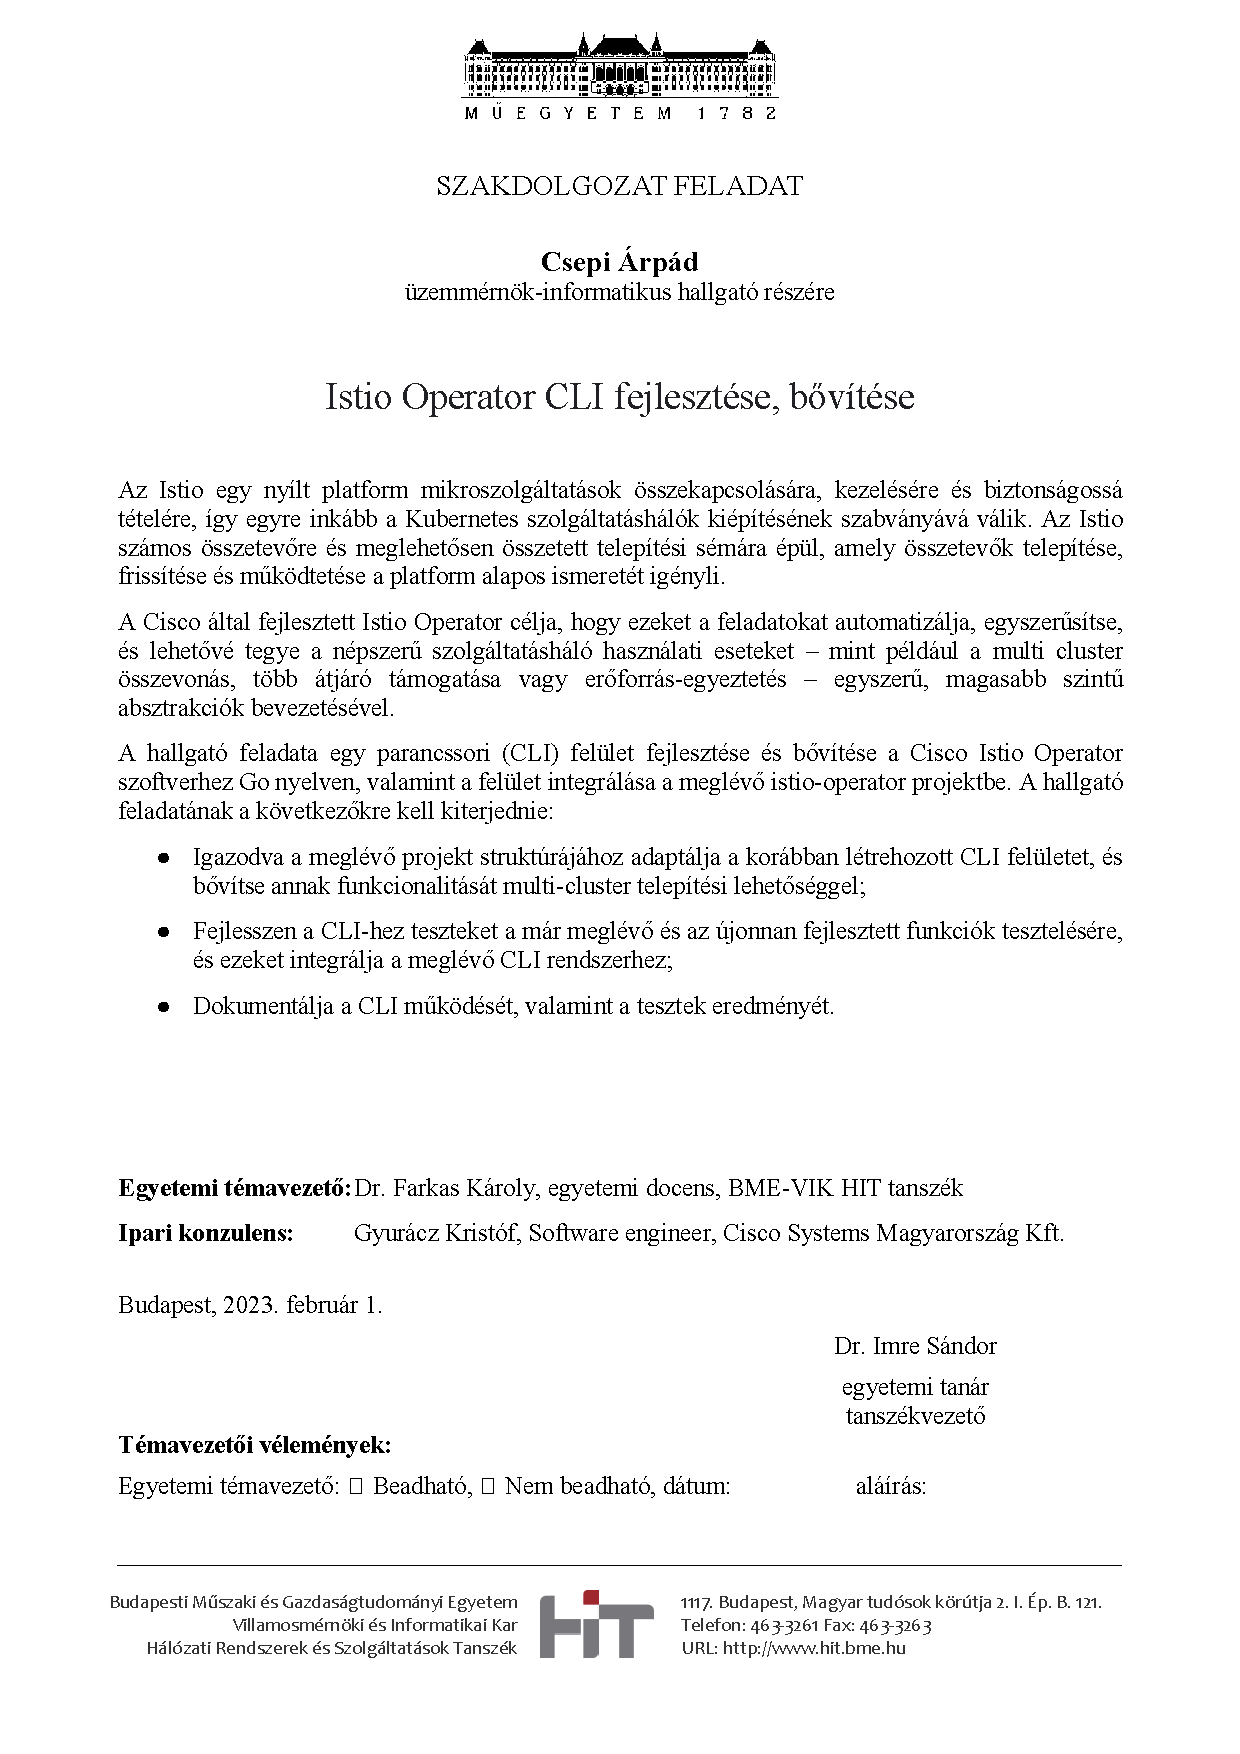
\includepdf[pages=-]{content/project/description.pdf}

% Table of Contents
%~~~~~~~~~~~~~~~~~~~~~~~~~~~~~~~~~~~~~~~~~~~~~~~~~~~~~~~~~~~~~~~~~~~~~~~~~~~~~~~~~~~~~~
\tableofcontents\vfill


% Declaration and Abstract
%~~~~~~~~~~~~~~~~~~~~~~~~~~~~~~~~~~~~~~~~~~~~~~~~~~~~~~~~~~~~~~~~~~~~~~~~~~~~~~~~~~~~~~
\selectlanguage{magyar}
\pagenumbering{gobble}
%--------------------------------------------------------------------------------------
% Nyilatkozat
%--------------------------------------------------------------------------------------
\begin{center}
\large
\textbf{HALLGATÓI NYILATKOZAT}\\
\end{center}

Alulírott \emph{\vikszerzoVezeteknev{} \vikszerzoKeresztnev}, szigorló hallgató kijelentem, hogy ezt a \vikmunkatipusat{} meg nem engedett segítség nélkül, saját magam készítettem, csak a megadott forrásokat (szakirodalom, eszközök stb.) használtam fel. Minden olyan részt, melyet szó szerint, vagy azonos értelemben, de átfogalmazva más forrásból átvettem, egyértelműen, a forrás megadásával megjelöltem.

Hozzájárulok, hogy a jelen munkám alapadatait (szerző(k), cím, angol és magyar nyelvű tartalmi kivonat, készítés éve, konzulens(ek) neve) a BME VIK nyilvánosan hozzáférhető elektronikus formában, a munka teljes szövegét pedig az egyetem belső hálózatán keresztül (vagy autentikált felhasználók számára) közzétegye. Kijelentem, hogy a benyújtott munka és annak elektronikus verziója megegyezik. Dékáni engedéllyel titkosított diplomatervek esetén a dolgozat szövege csak 3 év eltelte után válik hozzáférhetővé.

\begin{flushleft}
\vspace*{1cm}
Budapest, \today
\end{flushleft}

\begin{flushright}
 \vspace*{1cm}
 \makebox[7cm]{\rule{6cm}{.4pt}}\\
 \makebox[7cm]{\emph{\vikszerzoVezeteknev{} \vikszerzoKeresztnev}}\\
 \makebox[7cm]{hallgató}
\end{flushright}
\thispagestyle{empty}

\vfill
\clearpage
\thispagestyle{empty} % an empty page

\selectthesislanguage
 %TODO Hallgatói nyilatkozat -- TDK és OTDK esetén törlendő!
\pagenumbering{roman}
\setcounter{page}{1}

\selecthungarian

%----------------------------------------------------------------------------
% Abstract in Hungarian
%----------------------------------------------------------------------------
\chapter*{Kivonat}\addcontentsline{toc}{chapter}{Kivonat}

Ennek a szakdolgozatnak a célja, hogy ismertesse a mai világ nélkülözhetetlen felhőalapú számítástechnikai rendszerek automatizált telepítését, menedzselését és működését a Kubernetes szoftver segítségével, illetve ingyenes és nyílt forráskodú megoldást kínáljon ezekre. 

Az automatizált telepítés és klaszterek összekapcsolásának segítésére készítettem egy konzolos applikációt Go programozási nyelv segítségével. Ez a felhasználóbarát megoldás elősegíti, hogy több a téma iránt érdeklődő embereknek nyújton egy eszközt, ami könnyen használható, átlátható és módosítható.

A szakdolgozatom első szakaszában ismertetem azoknak a technológiáknak a hátterét, melyekre a program működésének megértéséhez szükség van.

Ezután bemutatom a programom tervezésének folyamatát, majd részletesen leírom az elkészített program szerkezeti felépítését és működését. Itt rávilágítok a program megvalósított funkcióira, a moduláris felépítésére, kiemelve a modulok legfontosabb részleteit. Bemutatom a tesztelési módszereket és dokumentálom az eredményeit.

A szakdolgozat végén összegzem a tanulságokat, elért eredményeket és további lehetséges fejlesztési lehetőségeket vázolok fel.

\vfill
\selectenglish


%----------------------------------------------------------------------------
% Abstract in English
%----------------------------------------------------------------------------
\chapter*{Abstract}\addcontentsline{toc}{chapter}{Abstract}

The purpose of this thesis is to describe the automated deployment, management and operation of cloud computing systems that are essential in today's world using Kubernetes software, and to provide a free and open-source solution for these. 

To help with automated deployment and cluster attaching, I created a console application using the Go programming language. This user-friendly solution helps to provide several people interested in the topic with a tool that is easy to use, transparent and modifiable.

In the first section of my thesis, I will describe the background of the technologies that are needed to understand how the program works.

I will then describe the process of designing my program, and then describe in detail the structure and operation of the program I have created. Here I will highlight the implemented features of the program, its modular structure, highlighting the most important details of the modules. I will present the testing methods and document the results.

At the end of the thesis, I summarise the lessons learned, the results achieved and outline further possible improvements.

\vfill
\selectthesislanguage

\newcounter{romanPage}
\setcounter{romanPage}{\value{page}}
\stepcounter{romanPage}    %TODO Összefoglaló -- TDK és OTDK esetén nem kötelező


% The main part of the thesis
%~~~~~~~~~~~~~~~~~~~~~~~~~~~~~~~~~~~~~~~~~~~~~~~~~~~~~~~~~~~~~~~~~~~~~~~~~~~~~~~~~~~~~~
\pagenumbering{arabic}

%TODO import your own content
%----------------------------------------------------------------------------
\chapter{\bevezetes}
%----------------------------------------------------------------------------

\paragraph{LaTeX minta ajánlása alapján}\mbox{}\smallskip

A bevezető tartalmazza a diplomaterv-kiírás elemzését, történelmi előzményeit, a feladat indokoltságát (a motiváció leírását), az eddigi megoldásokat, és ennek tükrében a hallgató megoldásának összefoglalását.

A bevezető szokás szerint a diplomaterv felépítésével záródik, azaz annak rövid leírásával, hogy melyik fejezet mivel foglalkozik.

\paragraph{TMIT GYIK ajánlása alapján}\mbox{}\smallskip

A bevezetés célja, hogy az olvasó válasz kapjon a következő kérdésekre:
\begin{itemize}
    \item hol helyezkedik el a téma a világban,
    \item mi a megoldandó feladat,
    \item mi teszi indokolttá a probléma kezelését,
    \item és a probléma megoldása mit tesz lehetővé a számunkra?
\end{itemize}

A fejezet végén, a diplomaterv felépítését foglald össze, minden fejezetről egy-egy bővített mondatot írj, hogy mivel fog foglalkozni a kérdéses szövegrész.

Annyira legyen részletes a bevezetés, hogy egy távközlési/informatikai alapműveltséggel rendelkező mérnök a bevezető alapján megértse, követni tudja a diplomafeladatod speciális problémáit. A legjobb teszt: add oda egy olyan évfolyamtársadnak, aki nem ismerős a diplomád témájában, és kérdezd meg, érti-e miről van szó!
%----------------------------------------------------------------------------
\chapter{\docker}
%----------------------------------------------------------------------------
\section{VMs vs containers}
\section{Docker}
%----------------------------------------------------------------------------
\chapter{\kubernetes}
%----------------------------------------------------------------------------
\section{Kubernetes bemutatása}
Láthattuk, hogy ahogy nő a rendszerben a telepíthető alkalmazáskomponensek száma, egyre nehezebb lesz mindegyiket kezelni.
A Google volt valószínűleg az első vállalat, amely felismerte, hogy sokkal jobb módszerre van szüksége a szoftverkomponensek telepítéséhez és kezeléséhez, valamint a globálisan skálázható infrastruktúrájához.
Egyike annak a kevés vállalatnak a világon, amely több százezer szervert üzemeltet, és amelynek a telepítések kezelésével kell foglalkoznia ilyen hatalmas léptékben.
Ez arra kényszerítette őket, hogy olyan megoldásokat dolgozzanak ki, amelyekkel több ezer szoftverkomponens fejlesztése és telepítése kezelhetővé és költséghatékonnyá tehető.

A Kubernetes egy olyan szoftverrendszer, amely lehetővé teszi, hogy egyszerűen telepítsünk és kezeljünk rajta konténeres alkalmazásokat.
A Linux konténerek funkcióira támaszkodik, hogy heterogén alkalmazásokat futtasson anélkül, hogy ismernie kellene ezen alkalmazások belső részleteit, és anélkül, hogy ezeket az alkalmazásokat manuálisan kellene telepíteni az egyes hosztokon.
Mivel ezek az alkalmazások konténerekben futnak, nem befolyásolják az ugyanazon a szerveren futó többi alkalmazást, ami kritikus fontosságú, ha teljesen különböző szervezetek alkalmazásait futtatja ugyanazon a hardveren.
Ez a felhőszolgáltatók számára kiemelkedő fontosságú, mivel a hardverük lehető legjobb kihasználására törekszenek, miközben a hosztolt alkalmazások teljes elszigeteltségét is fenn kell tartaniuk.
A Kubernetes lehetővé teszi, hogy szoftveralkalmazásait több ezer számítógépcsomóponton futtassa, mintha ezek a csomópontok mind egyetlen, hatalmas számítógép lenne.
Absztrahálja a mögöttes infrastruktúrát, és ezáltal egyszerűsíti a fejlesztést, a telepítést és a kezelést mind a fejlesztő, mind az üzemeltetési csapatok számára.
Az alkalmazások telepítése a Kubernetes segítségével mindig ugyanaz, függetlenül attól, hogy a klaszter (későbbiekben cluster) csak néhány csomópontot (későbbiekben node) tartalmaz vagy több ezret.
A cluster mérete egyáltalán nem számít.
A további node-ok egyszerűen a telepített alkalmazások számára rendelkezésre álló erőforrások további mennyiségét jelentik \cite{Marko17}.

\section{A Kubernetes működésének megértése}
A rendszer egy fő csomópontból (későbbiekben master node) és tetszőleges számú munkás csomópontból (későbbiekben worker node) áll.
Amikor a fejlesztő elküldi az alkalmazások listáját a master-nek, a Kubernetes telepíti azokat a worker node-okra (lásd \ref{kubernetes-overview} ábrán).
Az, hogy egy komponens melyik worker node-on landol, nem számít (és nem is szabadna számítania) sem a fejlesztőnek, sem a rendszergazdának.
A fejlesztő megadhatja, hogy bizonyos alkalmazásoknak együtt kell futniuk, és a Kubernetes ugyanarra a worker node-ra telepíti őket.
Mások szétszóródnak a cluster-ben, de ugyanúgy tudnak egymással kommunikálni, függetlenül attól, hogy hova telepítik őket \cite{Marko17}.

\begin{figure}[ht]
    \centering
         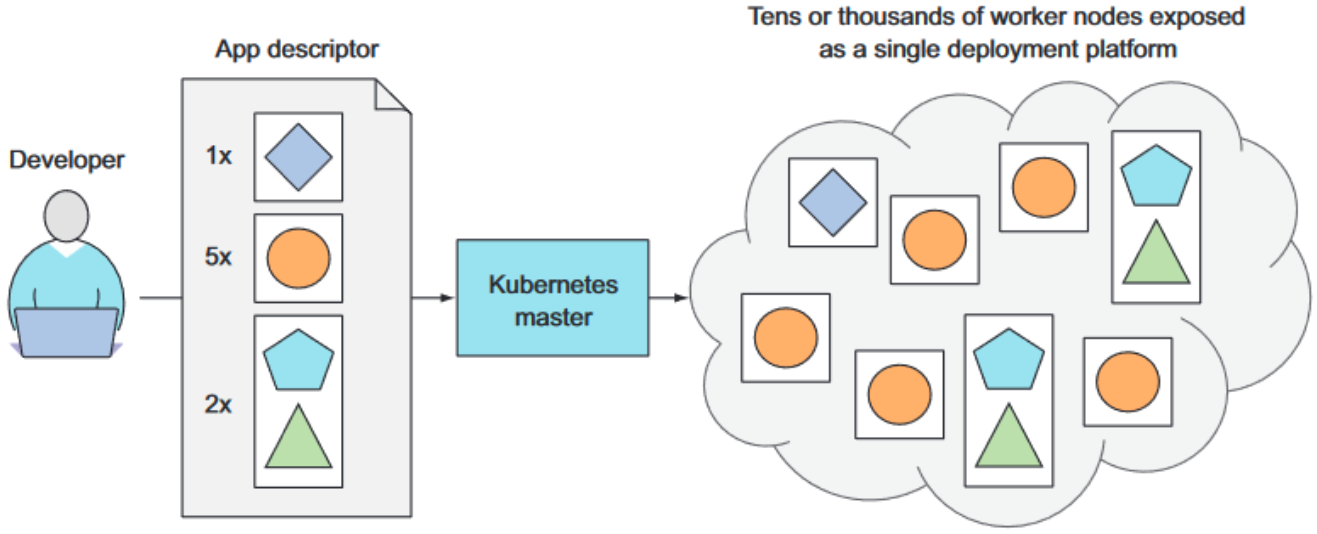
\includegraphics[width=1.0\textwidth]{figures/kubernetes/kubernetes-overview.png}
          \caption{A Kubernetes, mint egyetlen telepítési platform \cite{Marko17}.}
           \label{kubernetes-overview}
\end{figure}

Hardveres szinten egy Kubernetes cluster sok node-ból áll, amelyek két típusra oszthatók:
\begin{itemize}
    \item A master node, amely a Kubernetes vezérlőjének (későbbiekben Control Plane) ad otthont, amely az egész Kubernetes rendszert irányítja és kezeli.
    \item A worker node, amely a tényleges telepített alkalmazásokat futtatja.
\end{itemize}

\newpage

\subsection{A Control Plane}
A Control Plane az, ami a cluster-t irányítja és működésre készteti.
Több komponensből áll, amelyek egyetlen master node-on futhatnak, vagy több node-ra oszthatók és replikálhatók a magas rendelkezésre állás biztosítása érdekében.
Ezek az összetevők a következők:
\begin{itemize}
    \item Az API szerver, amellyel a felhasználó és a többi control plane komponens kommunikál.
    \item Az ütemező (későbbiekben Scheduler), amely ütemezi az alkalmazásokat (az alkalmazás minden telepíthető komponenséhez hozzárendel egy worker node-ot).
    \item A vezérlő menedzser (későbbiekben Controller Manager), amely cluster szintű funkciókat lát el, mint például a komponensek replikálása, a munkás node-ok nyomon követése, a node-ok hibáinak kezelése stb.
    \item etcd, egy megbízható elosztott adattároló, amely tartósan tárolja a cluster konfigurációját.
\end{itemize}
A Control Plane összetevői tartják és vezérlik a cluster állapotát, de nem futtatják az alkalmazásokat (lásd \ref{cluster-overview} ábrán). Ezt a worker node-ok végzik \cite{Marko17}.

\subsection{A worker node-ok}
A worker node-ok azok a gépek, amelyek a konténerizált alkalmazásokat futtatják (lásd \ref{cluster-overview} ábrán).
Az alkalmazások futtatásának, felügyeletének és szolgáltatásnyújtásának feladatát a következő komponensek végzik: \cite{Marko17}
\begin{itemize}
    \item Docker, rkt vagy más konténer futtató, amely futtatja a konténereket.
    \item A Kubelet kommunikál az API-kiszolgálóval és kezeli a konténereket a node-ján.
    \item A Kubernetes Service Proxy (kube-proxy), amely elosztja a hálózati forgalmat az alkalmazáskomponensek között.
\end{itemize}

\begin{figure}[ht]
    \centering
         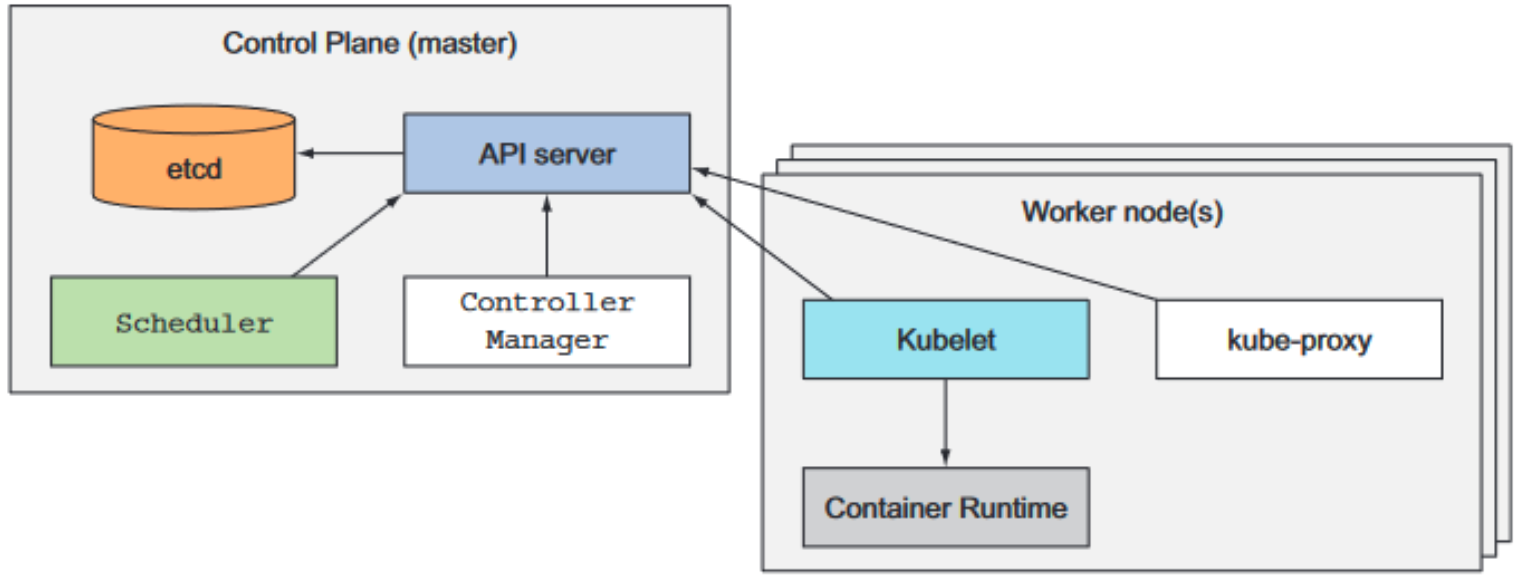
\includegraphics[width=1.0\textwidth]{figures/kubernetes/cluster-overview.png}
          \caption{A Kubernetes cluster-t alkotó komponensek \cite{Marko17}.}
           \label{cluster-overview}
\end{figure}

\subsection{A podok bevezetése}
A Kubernetes nem foglalkozik közvetlenül az egyes konténerekkel.
Ehelyett a több, együtt elhelyezett konténer koncepcióját használja.
Ezt a konténerekből álló csoportot podnak nevezzük.
A pod egy vagy több szorosan összefüggő konténer csoportja, amelyek mindig ugyanazon a worker node-on és ugyanazon a linux névtereken futnak együtt.
Minden pod olyan, mint egy különálló logikai gép, saját IP-vel, hostnévvel, folyamatokkal, amely egyetlen alkalmazást futtat (lásd \ref{node-pod-scheduler} ábrán).
Az alkalmazás lehet egyetlen folyamat, amely egyetlen konténerben fut, vagy lehet egy fő alkalmazási folyamat és további támogató folyamatok, amelyek mindegyike saját konténerben fut.
Egy podban lévő összes konténer látszólag ugyanazon a logikai gépen fut, míg a többi podban lévő konténerek, még ha ugyanazon a worker node-on futnak is, látszólag másikon futnak \cite{Marko17}.

\begin{figure}[ht]
    \centering
         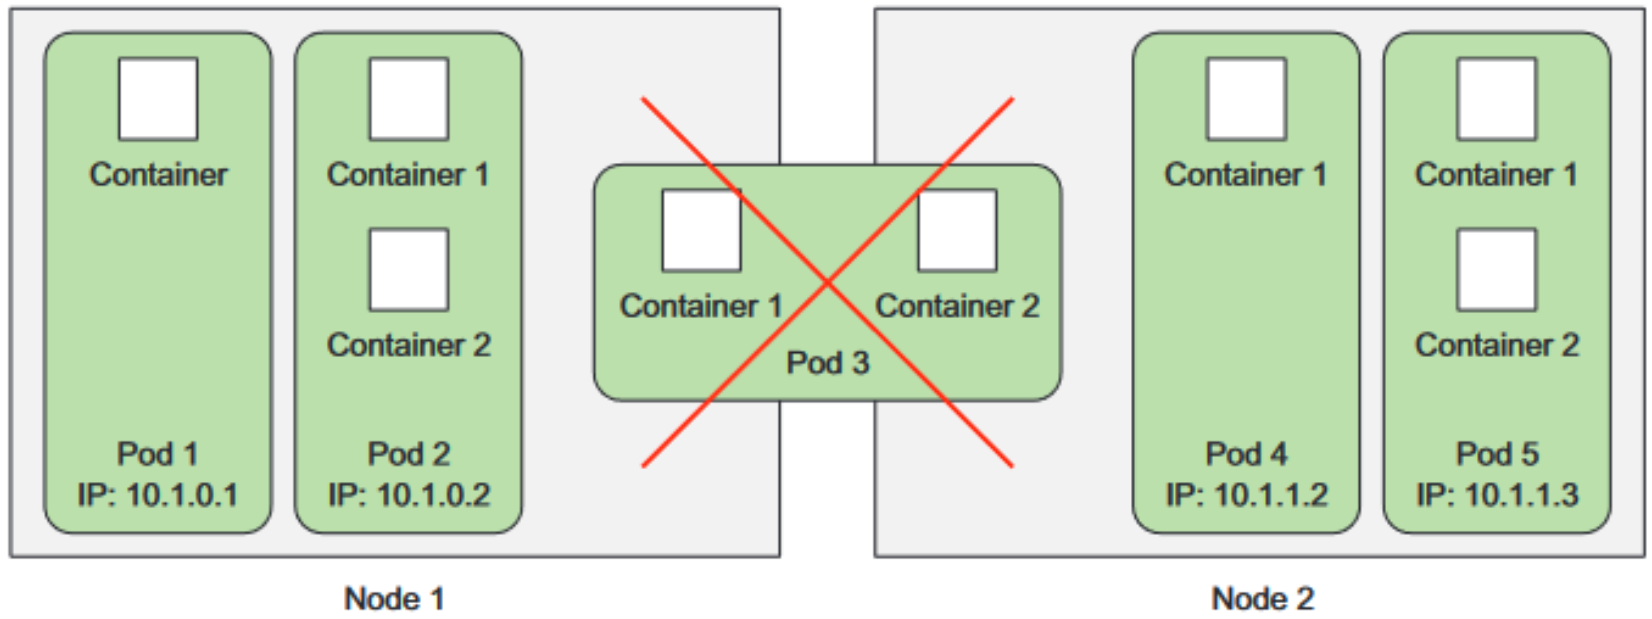
\includegraphics[width=1.0\textwidth]{figures/kubernetes/node-pod-scheduler.png}
          \caption{Egy pod minden konténere ugyanazon a node-on fut. Egy pod soha nem terjed ki két node-ra \cite{Marko17}.}
           \label{node-pod-scheduler}
\end{figure}

\subsection{A Service bemutatása}
A Kubernetes Service egy olyan erőforrás, amelyet azért hozunk létre, hogy egyetlen, állandó belépési pont legyen egy podok csoportjához, amelyek ugyanazt a szolgáltatást nyújtják.
Minden szolgáltatásnak van egy IP-címe és portja, amelyek a szolgáltatás létezése alatt soha nem változik.
Az felhasználók kapcsolatot nyithatnak az adott IP-címre és portra és ezek a kapcsolatok az adott szolgáltatást támogató podok egyikéhez kerülnek továbbításra.
Így a szolgáltatás felhasználóinak nem kell ismerniük a szolgáltatást nyújtó egyes podok helyét és címét, így ezek a podok bármikor áthelyezhetők a cluter-en belül (lásd \ref{service-overview} ábrán) \cite{Marko17}.

\begin{figure}[ht]
    \centering
         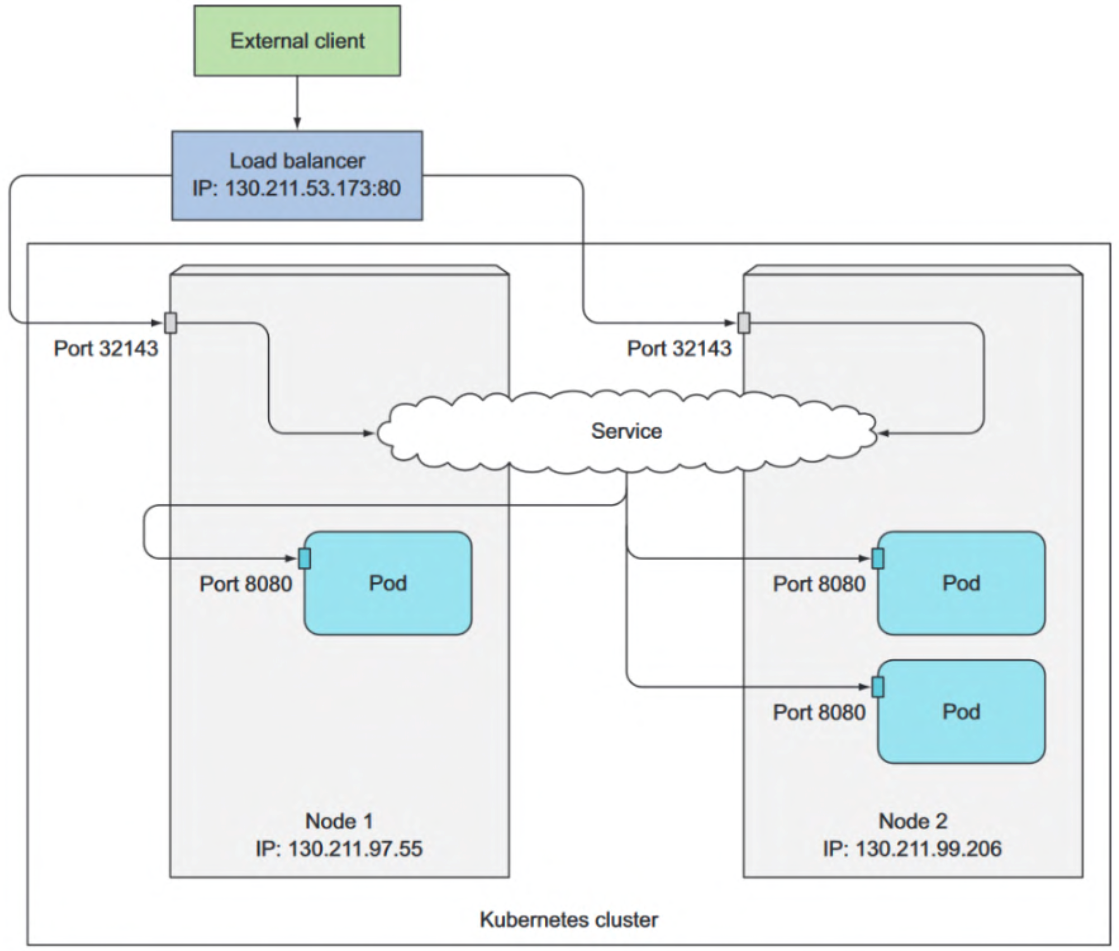
\includegraphics[width=0.9\textwidth]{figures/kubernetes/service-overview.png}
          \caption{Szolgáltatás megnyitása külső felhasználók számára \cite{Marko17}.}
           \label{service-overview}
\end{figure}

\subsection{A Secrets bemutatása}
A konfiguráció általában érzékeny információkat is tartalmaz, például hitelesítő adatokat és privát titkosítási kulcsokat, amelyeket biztonságban kell tartani.
Az ilyen információk tárolására és terjesztésére a Kubernetes egy különálló objektumot biztosít, amelyet Secretnek hívnak.
A titkok hasonlóak a ConfigMaps-hoz, ők is leképezések, amelyek kulcs-érték párokat tartalmaznak.
A Kubernetes segít megőrizni a Secrets biztonságát azzal, hogy minden Secret csak azokhoz a node-okhoz jut el, amelyek a Secret hozzáférésre szoruló podokat futtatják.
Emellett a node-okon maguk a Secret-ek mindig a memóriában tárolódnak, és soha nem íródnak fizikai tárolókra, ami a lemezek törlését igényelné a Secret törlése után. Magán a master node-on (pontosabban az etcd-ben) a Secret-eket korábban titkosítatlan formában tárolták, ami azt jelentette, hogy a master node-ot védeni kell az tárolt érzékeny adatok biztonsága érdekében.
Ez nem csak az etcd tárolás biztonságban tartására terjedt ki, hanem arra is, hogy megakadályozzuk, hogy illetéktelen felhasználók használhassák az API-kiszolgálót, mivel bárki, aki podokat tud létrehozni, fel tudja csatolni a secret-et a podba, és azon keresztül hozzáférhet az érzékeny adatokhoz.
A Kubernetes 1.7-es verziójától az etcd titkosított formában tárolja a Secret-eket, ami sokkal biztonságosabbá teszi a rendszert \cite{Marko17}.

\subsection{Kliens könyvtárak az API-kiszolgálóval való kommunikációhoz}
A Kubernetes közösségnek számos speciális érdekcsoportja és munkacsoportja van, amelyek a Kubernetes ökoszisztéma egyes részeire összpontosítanak.
Jelenleg két Kubernetes API klienskönyvtár létezik, amelyeket az API Machinery speciális érdekcsoport (SIG) támogat: \cite{Marko17}

\begin{itemize}
    \item Golang client (https://github.com/kubernetes/client-go)
    \item Python (https://github.com/kubernetes-incubator/client-python)
\end{itemize}

\subsection{Egyéni API-objektumok definiálása}
Ahogy a Kubernetes ökoszisztéma fejlődik, egyre több és több magas szintű objektumot fog látni, amelyek sokkal speciálisabbak lesznek, mint a Kubernetes által ma támogatott erőforrások.
Ahelyett, hogy Deployments, Services, ConfigMaps és hasonlókkal foglalkozna, egész alkalmazásokat vagy szoftverszolgáltatásokat reprezentáló objektumokat fog létrehozni és kezelni.

Egy egyéni vezérlő fogja megfigyelni ezeket a magas szintű objektumokat, és ezek alapján alacsony szintű objektumokat hoz létre.
Például ahhoz, hogy a webhelyobjektumok egy szolgáltatáson keresztül elérhető webkiszolgáló podot futtassanak, létre kell hoznia és telepítenie kell egy webhelyvezérlőt, amely figyeli az API-kiszolgálót a webhelyobjektumok létrehozására, majd létrehozza a szolgáltatást és a webkiszolgáló podot mindegyikhez (lásd \ref{custom-controller} ábrán).
Annak érdekében, hogy a Pod kezelt legyen és túlélje a node-ok hibáit, a vezérlő közvetlenül egy deployment erőforrást hoz létre a nem kezelt pod helyett \cite{Marko17}.

\begin{figure}[ht]
    \centering
         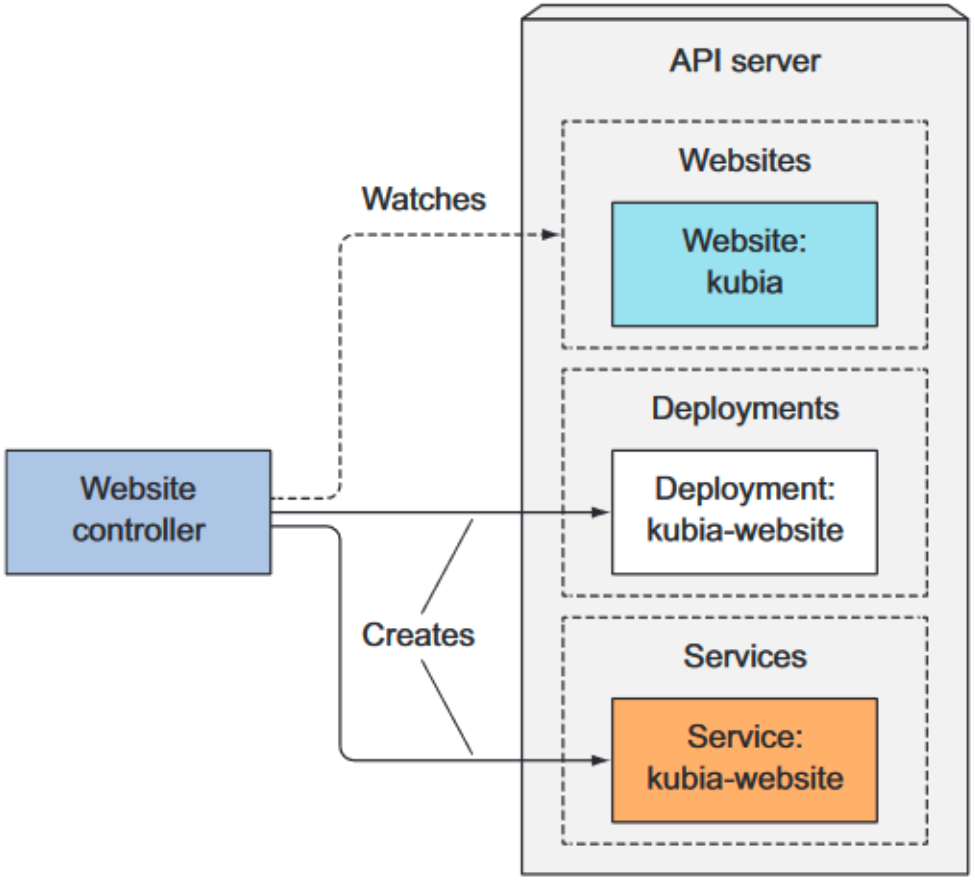
\includegraphics[width=0.85\textwidth]{figures/kubernetes/custom-controller.png}
          \caption{A weboldal controllere figyeli a webhely objektumokat és létrehoz egy deployment-et és egy service-t \cite{Marko17}.}
           \label{custom-controller}
\end{figure}

\newpage

\subsection{Az operátor bemutatása}
Az operátor egy Kubernetes-alkalmazás csomagolására, telepítésére és kezelésére szolgáló módszer. Egy Kubernetes-alkalmazást egyszerre telepítünk a Kubernetesre és kezelünk a Kubernetes API (alkalmazásprogramozási felület) és a kubectl tool (segédeszköz) segítségével.

A Kubernetes-operátor egy alkalmazásspecifikus vezérlő, amely a Kubernetes API funkcionalitását kiterjeszti, hogy komplex alkalmazások példányait hozza létre, konfigurálja és kezelje a Kubernetes-felhasználó nevében.
A Kubernetes erőforrás és vezérlő alapkoncepcióira épül, de magában foglalja a tartomány- vagy alkalmazásspecifikus tudást az általa kezelt szoftver teljes életciklusának automatizálása érdekében. 

A Kubernetesben a control plane vezérlői olyan vezérlési feladatokat valósítanak meg, amelyek ismételten összehasonlítják a cluster kívánt állapotát annak tényleges állapotával.
Ha a cluster tényleges állapota nem egyezik a kívánt állapottal, akkor a vezérlő lépéseket tesz a probléma kijavítására. 

Az operátor egy olyan egyéni Kubernetes vezérlő, amely egyéni erőforrást (későbbiekben custom resource vagy CR) használ az alkalmazások és komponenseik kezelésére.
A magas szintű konfigurációt és beállításokat a felhasználó adja meg egy custom resource-on belül.
A Kubernetes operátor a magas szintű utasításokat az operátor logikájába ágyazott legjobb gyakorlatok alapján fordítja le az alacsony szintű műveletekre.

A custom resource Kubernetes API-bővítési mechanizmusa.
Egy egyéni erőforrás-definíció (későbbiekben custom resource definition vagy CRD) definiál egy CR-t, és felsorolja az operátor felhasználói számára elérhető összes konfigurációt.
A Kubernetes-operátor figyeli a CR típusát, és alkalmazásspecifikus műveleteket hajt végre annak érdekében, hogy az aktuális állapot megfeleljen az erőforrás által kívánt állapotának.

A Kubernetes-operátorok új objektumtípusokat vezetnek be az CRD-k révén.
A CRD-t a Kubernetes API ugyanúgy kezelheti, mint a beépített objektumokat, beleértve a kubectl-en keresztüli interakciót és a szerepkör-alapú hozzáférés-szabályozásba (RBAC) való felvételt.
Az operátor továbbra is figyelemmel kíséri az alkalmazását, miközben az fut, és automatikusan biztonsági mentést készíthet az adatokról, helyreállíthatja a hibákat, és frissítheti az alkalmazást. 

A Kubernetes-operátor által végzett műveletek szinte bármi lehet: egy összetett alkalmazás skálázása, az alkalmazás verziófrissítése, vagy akár egy speciális hardverrel rendelkező számítási cluster node-jainak kernelmoduljainak kezelése \cite{RedHatKubOp}.

Az Istio operátor felépítése látható \ref{operator-overview} ábrán.

\newpage

\section{Kubernetes in Docker}
A Kubernetes in Docker (későbbiekben kind) egy eszközcsomag a helyi Kubernetes cluster-ekhez, ahol minden node egy Docker konténer. A kind a Kubernetes tesztelését célozza meg.

A kind funkcionalitásának nagy részét megvalósító go csomagokra, a felhasználóknak szánt parancssorra és egy node base image-re (alap lemezképre) oszlik. A szándék az, hogy a kind csomagjai importálható és újrafelhasználható legyen más eszközök (pl. kubetest) által, míg a CLI gyors módot biztosít e csomagok használatára és hibakeresésére.

Bár nem minden tesztelés végezhető el valódi cluster-ek nélkül a felhőben, de elég lehet ahhoz, hogy ha valami ilyesmit akarunk: \cite{KinD}
\begin{itemize}
    \item Nagyon olcsó cluster-eket futtatni, amelyeket bármely fejlesztői környezetben replikálhatóak.
    \item Integrálható más eszközökkel.
    \item Aslaposan dokumentált és karbantartható.
    \item Nagyon stabil, kiterjedt hibakezeléssel rendelkezik.
\end{itemize}

A kind működését \ref{kind-overview} ábra tartalmazza.

\begin{figure}[ht]
    \centering
         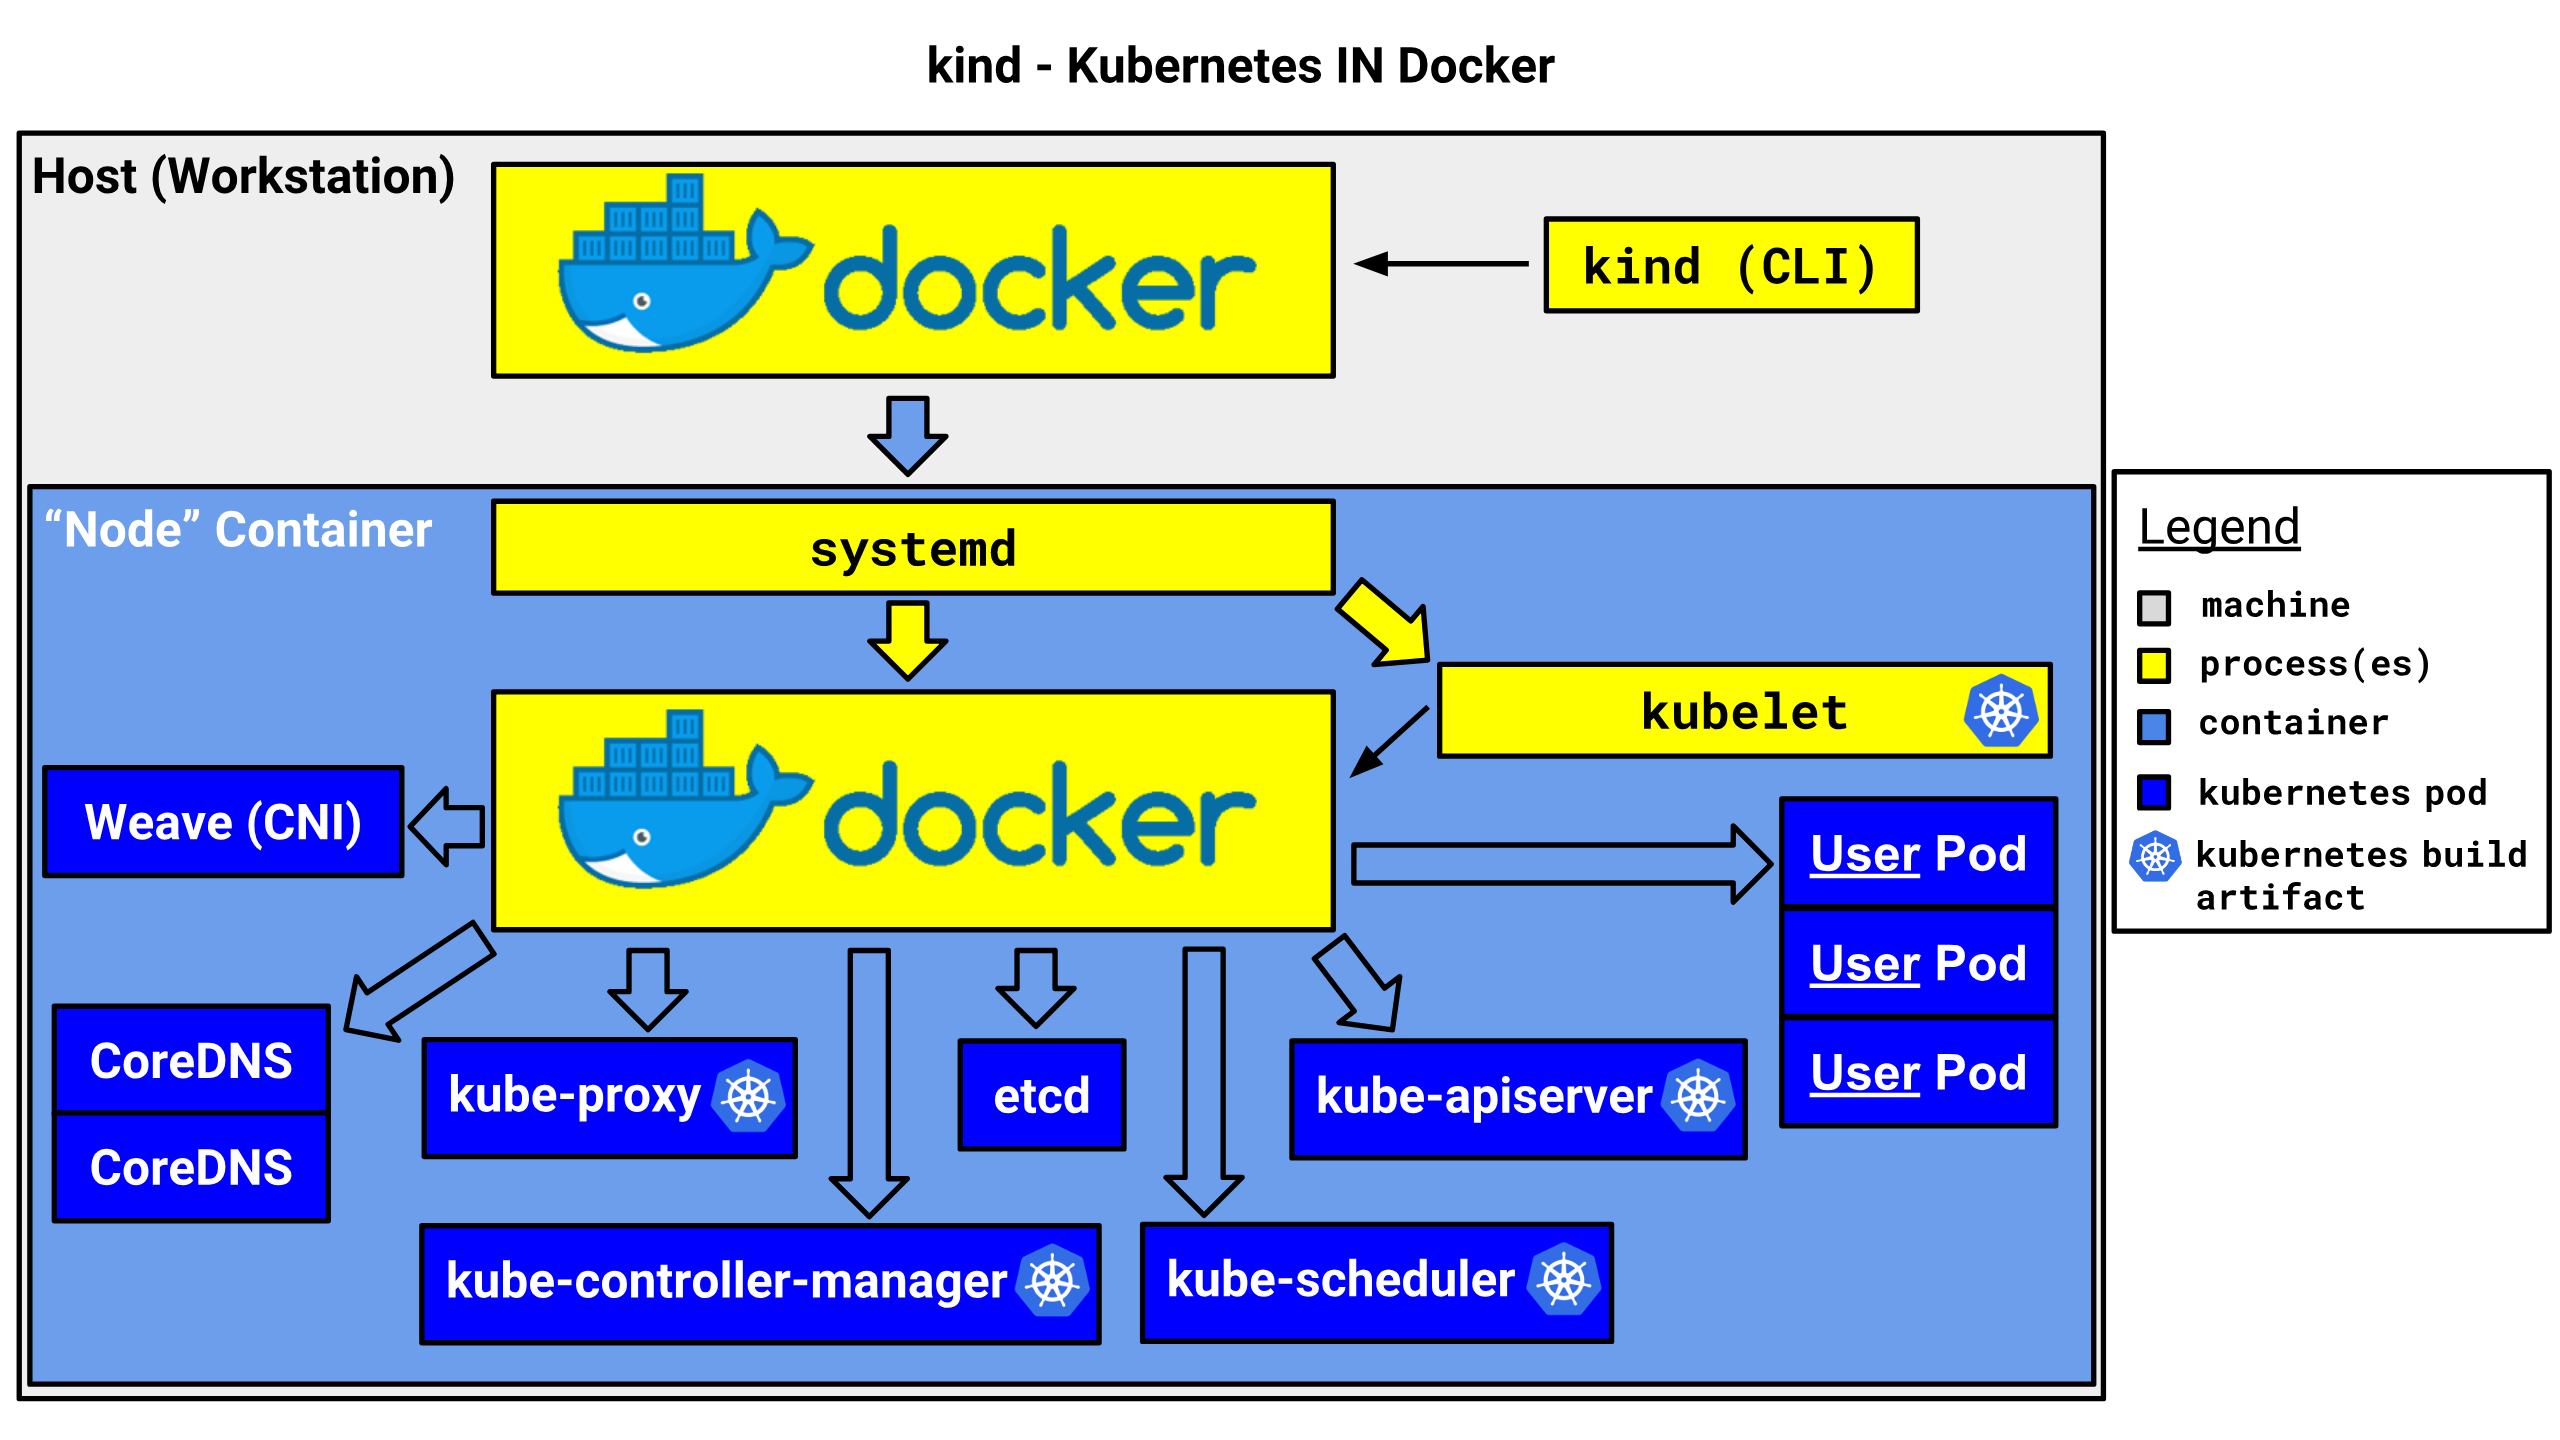
\includegraphics[width=0.85\textwidth]{figures/kubernetes/kind-overview.png}
          \caption{KinD felépítése a gyakorlatban \cite{KinD}.}
           \label{kind-overview}
\end{figure}
%----------------------------------------------------------------------------
\chapter{\istio}
%----------------------------------------------------------------------------
\section{Istio}
\section{Istio operátor}
\section{Banzaicloud istio operátor}
\subsection{Multi cluster}
%----------------------------------------------------------------------------
\chapter{\golang}
%----------------------------------------------------------------------------
\section{Szintaktika}
\section{Csomagkezelő}
\section{Tesztelés}
%----------------------------------------------------------------------------
\chapter{\github}
%----------------------------------------------------------------------------
\section{Git}
A verziókezelő rendszer (későbbiekben Version Control System vagy VCS) nyomon követi a változtatások történetét, ahogy az emberek és a csapatok együtt dolgoznak a projekteken.
Ahogy a fejlesztők változtatásokat végeznek a projekten, a projekt bármely korábbi verziója bármikor visszaállítható.

A fejlesztők áttekinthetik a projekttörténetet, hogy megtudják:
\begin{itemize}
  \item Milyen változtatásokat végeztek.
  \item Ki végezte a változtatásokat.
  \item Mikor történtek a változtatások.
  \item Miért volt szükség a változtatásokra.
\end{itemize}

A VCS-ek minden egyes közreműködőnek egységes és konzisztens képet adnak a projektről, felszínre hozva a már folyamatban lévő munkát.
A változtatások átlátható előzményeinek, a változtatásokat végző személyeknek és a projekt fejlődéséhez való hozzájárulásuknak a megtekintése segít a csapattagoknak abban, hogy a független munka során is összhangban maradjanak.

Egy elosztott verziókezelő rendszerben (későbbiekben Distributed Version Control System vagy DVCS) minden fejlesztő rendelkezik a projekt és a projekttörténet teljes másolatával.
Az egykor népszerű központosított verziókezelő rendszerekkel ellentétben a DVCS-eknek nincs szükségük állandó kapcsolatra egy központi adattárral.

\newpage

A Git a legnépszerűbb elosztott verziókezelő rendszer. A Git-et gyakran használják nyílt forráskódú és kereskedelmi szoftverfejlesztésre egyaránt, és jelentős előnyökkel jár az egyének, a csapatok és a vállalkozások számára:
\begin{itemize}
  \item A Git segítségével a fejlesztők egy helyen láthatják a változtatások, döntések és a projekt előrehaladásának teljes idővonalát. Attól a pillanattól kezdve, hogy hozzáférnek egy projekt előzményeihez, a fejlesztő minden szükséges kontextussal rendelkezik ahhoz, hogy megértse azt, és elkezdjen hozzájárulni.
  \item A fejlesztők minden időzónában dolgoznak. Egy olyan DVCS-vel, mint a Git, az együttműködés bármikor megtörténhet, miközben a forráskód integritása megmarad. Az ágak használatával a fejlesztők biztonságosan javasolhatnak változtatásokat a termelési kódhoz.
  \item A Git-et használó vállalkozások lebonthatják a csapatok közötti kommunikációs akadályokat, és a csapatok a legjobb munkájukra koncentrálhatnak. Ráadásul a Git lehetővé teszi, hogy az egész vállalat szakértői együttműködjenek a nagyobb projektekben.
\end{itemize}

A repository vagy Git-projekt a projekthez tartozó fájlok és mappák teljes gyűjteményét foglalja magában, az egyes fájlok revíziós előzményeivel együtt.
A fájlok előzményei időbeli pillanatképek formájában jelennek meg, amelyeket commitoknak nevezünk.
A commitok több fejlesztési sorba, úgynevezett ágakba szervezhetők. Mivel a Git egy DVCS, a tárolók önálló egységek, és bárki, aki rendelkezik a tároló másolatával, hozzáférhet a teljes kódbázishoz és annak történetéhez.
A parancssor vagy más egyszerű kezelőfelületek használatával a Git-tár lehetővé teszi a következőket is: interakció az előzményekkel, a tár klónozása, ágak létrehozása, átadás, beolvasztás, összevonás, a kódverziók közötti változások összehasonlítása stb.

Az olyan platformokon keresztül, mint a GitHub, a Git több lehetőséget biztosít a projektek átláthatóságára és együttműködésére is.
A nyilvános adattárak segítik a csapatok együttműködését a lehető legjobb végtermék létrehozásában \cite{git}.

\section{GitHub}
A GitHub egy olyan fejlesztési platform, amely lehetővé teszi a kódok tárolását és felülvizsgálatát, a projektek kezelését és a szoftverek készítését 50 millió fejlesztővel együttműködve.
Miért épít mindenki a GitHubra? Mert biztosítja azokat a fontos DevOps funkciókat, amelyekre a vállalatoknak és a különböző méretű szervezeteknek szükségük van a nyilvános és magánprojektjeikhez.
Legyen szó funkciók tervezéséről, hibák javításáról vagy a változtatásokon való együttműködésről, a GitHub az a hely, ahol a világ szoftverfejlesztői összegyűlnek, hogy dolgokat hozzanak létre és aztán jobbá teszik őket.
A GitHub egy felhőplatform, amely a Git-et használja alapvető technológiaként.
Leegyszerűsíti a projekteken való együttműködés folyamatát, és olyan weboldalt, parancssori eszközöket és általános folyamatot biztosít, amely lehetővé teszi a fejlesztők és a felhasználók közös munkáját.

\subsection{GitHub Actions ismertető}
A GitHub Actions egy folyamatos integrációs és folyamatos szállítási (későbbiekben CI/CD) platform, amely lehetővé teszi, hogy automatizálja a build, a tesztelés és a telepítés folyamatot.
Létrehozhat olyan munkafolyamatokat (későbbiekben workflow), amelyek minden egyes pull-kérelem után build-el és tesztel a tárolóban (későbbiekben repository).

A GitHub Actions túlmutat a DevOps-on, és lehetővé teszi, hogy workflow-kat futtasson, amikor más események is történnek a tárolóban.
Például futtathat olyan workflow-t, amely automatikusan hozzáadja a megfelelő címkéket, amikor valaki új problémát (későbbiekben issue) hoz létre az respository-ban.

A GitHub Linux, Windows és macOS virtuális gépeket biztosít a workflow-ok futtatásához, de saját adatközpontban vagy felhő-infrastruktúrában is hosztolhatsz saját, saját üzemeltetésű futásokat (későbbiekben runner) \cite{github}.

\subsection{A GitHub Actions elemei}
Konfigurálhat egy GitHub Actions workflow-t, amely akkor indul el, amikor egy esemény történik a repository-ban, például egy pull request megnyitásakor vagy egy issue létrehozásakor.
A workflow egy vagy több feladatot tartalmaz, amelyek futhatnak egymás utáni sorrendben vagy párhuzamosan (lásd \ref{overview-actions-simple} ábrán).
Minden egyes feladat a saját virtuális gépi runner-jén vagy egy konténeren belül fut, és egy vagy több lépésből áll, amelyek vagy egy általad definiált szkriptet futtatnak, vagy egy műveletet futtatnak, ami egy újrafelhasználható bővítmény, amely egyszerűsítheti a workflow-t \cite{github}.

\begin{figure}[ht]
    \centering
         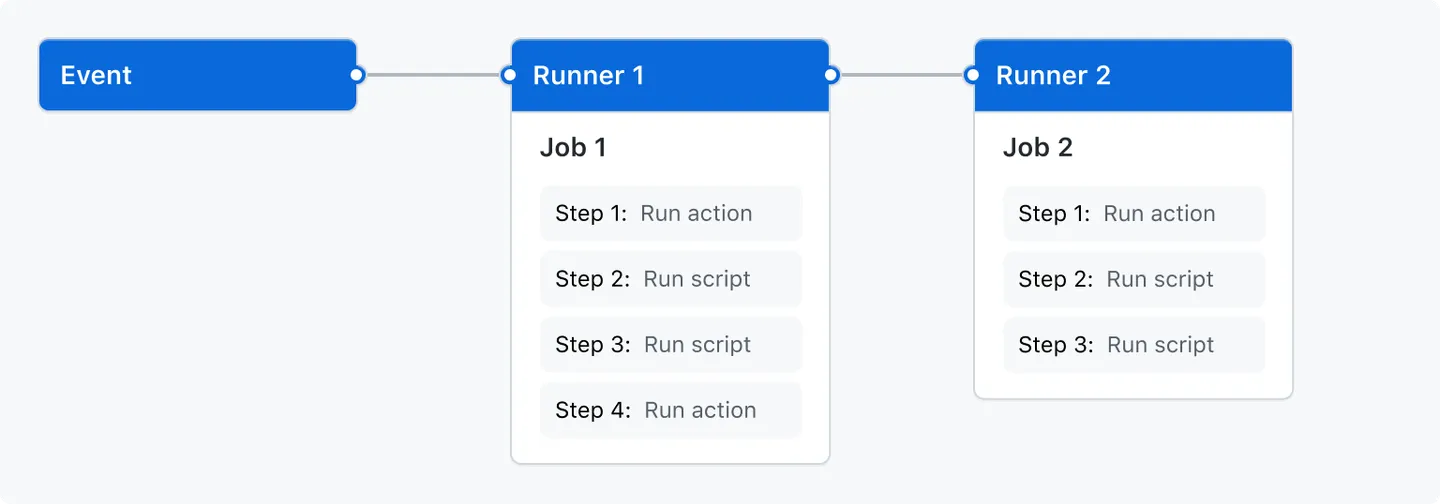
\includegraphics[width=1.0\textwidth]{figures/github/overview-actions-simple.png}
          \caption{Egy esemény diagramja, amely az 1. runner-t az 1. feladat futtatására indítja, ami a 2. runner-t a 2. feladat futtatására indítja. Mindegyik feladat több lépésre van bontva \cite{github}.}
           \label{overview-actions-simple}
\end{figure}

\subsubsection*{Workflows}
A workflow egy konfigurálható automatizált folyamat, amely egy vagy több feladatot futtat. A workflow-kat az repository-ba bevitt YAML fájl határozza meg, és akkor futnak, amikor az repository-ban lévő esemény kiváltja őket, vagy manuálisan, illetve meghatározott ütemezés szerint is elindíthatók.

A workflow-k a .github/workflows könyvtárban vannak definiálva egy repository-ban, és egy repository-hoz több workflow is tartozhat, amelyek mindegyike más-más feladatokat végezhet.
Például lehet egy workflow a pull-kérelmek létrehozására és tesztelésére, egy másik workflow az alkalmazás telepítésére minden egyes kiadás létrehozásakor, és még egy másik workflow, amely minden egyes alkalommal hozzáad egy címkét, amikor valaki új issue-t nyit. Hivatkozhat egy workflow-ra egy másik workflow-on belül \cite{github}.

\subsubsection*{Events}
Az esemény (event) egy konkrét tevékenység egy repository-ban, amely egy workflow végrehajtását indítja el.
Az aktivitás például a GitHubról származhat, amikor valaki létrehoz egy pull requestet, megnyit egy issue-et, vagy egy commit-ot küld a repositoryba. A workflow-t időzítéssel, REST API-ba való beküldéssel vagy manuálisan is elindíthatja \cite{github}.

\subsubsection*{Jobs}
A feladat (job) egy workflow lépéseinek olyan csoportja, amelyet ugyanazon a runner-en hajtanak végre.
Minden lépés vagy egy végrehajtandó shell szkript, vagy egy végrehajtandó művelet.
A lépések sorrendben kerülnek végrehajtásra, és egymástól függnek. Mivel minden lépés ugyanazon a futón kerül végrehajtásra, az adatokat megoszthatja egyik lépésről a másikra. Például lehet egy lépés, amely elkészíti az alkalmazást, majd egy lépés, amely teszteli a felépített alkalmazást.

Beállíthatja egy feladat függőségeit más feladatokkal; alapértelmezés szerint a feladatoknak nincsenek függőségeik, és párhuzamosan futnak egymással.
Ha egy feladat függőséget vesz fel egy másik feladattól, akkor megvárja a függő feladat befejezését, mielőtt lefuthatna. Lehet például több, különböző architektúrákhoz tartozó építési feladat, amelyek nem függnek egymástól, és egy csomagolási feladat, amely függ ezektől a feladatoktól.
A build feladatok párhuzamosan futnak, és ha mindegyik sikeresen befejeződött, akkor a csomagolási feladat is lefut \cite{github}.

\subsubsection*{Actions}
A művelet (action) a GitHub Actions platform egyéni alkalmazása, amely egy összetett, de gyakran ismétlődő feladatot hajt végre.
Egy művelet használatával csökkentheti a workflow fájlokban írt ismétlődő kód mennyiségét.
Egy művelet lehívhatja a git-tárat a GitHubról, beállíthatja a megfelelő eszköztárat az build környezetéhez, vagy beállíthatja a hitelesítést a felhőszolgáltatónál.

Írhat saját műveleteket, vagy találhat workflow-okhoz felhasználható műveleteket a GitHub Marketplace-en \cite{github}.

\subsubsection*{Runners}
A futtató (későbbiekben runner) egy olyan kiszolgáló, amely a workflow-okat futtatja, amikor azoknak el kell elindulniuk.
Minden runner egyszerre egyetlen feladatot futtathat.
A GitHub Ubuntu Linux, Microsoft Windows és macOS runnereket biztosít a workflow-ok futtatásához; minden workflow futtatása egy friss, újonnan rendelkezésre bocsátott virtuális gépen történik.
A GitHub nagyobb futókat is kínál, amelyek nagyobb konfigurációkban állnak rendelkezésre \cite{github}.

\subsubsection*{Egy példa workflow}
A GitHub Actions YAML szintaxist használ a workflow-ok meghatározásához.
Minden workflow különálló YAML-fájlként tárolódik a kódtárában, a .github/workflows nevű könyvtárban.

Létrehozhat egy példát a repository-jában ahogyan a \ref{sample-actions-config} ábrán is látható, amely automatikusan elindít egy sor parancsot, amikor kódot küldünk be.
Ebben a workflow-ban a GitHub Actions ellenőrzi a beküldött kódot, telepíti a bats tesztelési keretrendszert, és lefuttat egy alapvető parancsot a bats verziójának kiadására: bats -v \cite{github}.

\begin{figure}
  \centering
    \begin{minipage}{\linewidth}
      \begin{lstlisting}
          name: learn-github-actions
          run-name: ${{ github.actor }} is learning GitHub Actions
          on: [push]
          jobs:
            check-bats-version:
              runs-on: ubuntu-latest
              steps:
                - uses: actions/checkout@v3
                - uses: actions/setup-node@v3
                  with:
                    node-version: '14'
                - run: npm install -g bats
                - run: bats -v
      \end{lstlisting}
      \end{minipage}
  \caption{Példa kód a GitHub Actions használatára \cite{github}.}
  \label{sample-actions-config}
\end{figure}

A \ref{overview-actions-event} ábrán látható az imént létrehozott példa workflow fájl, valamint a GitHub Actions összetevőinek hierarchikus elrendezése.
Minden lépés egyetlen műveletet vagy szkriptet hajt végre.
Az 1. és 2. lépés műveleteket, míg a 3. és 4. lépés szkripteket futtat.

\begin{figure}[ht]
    \centering
         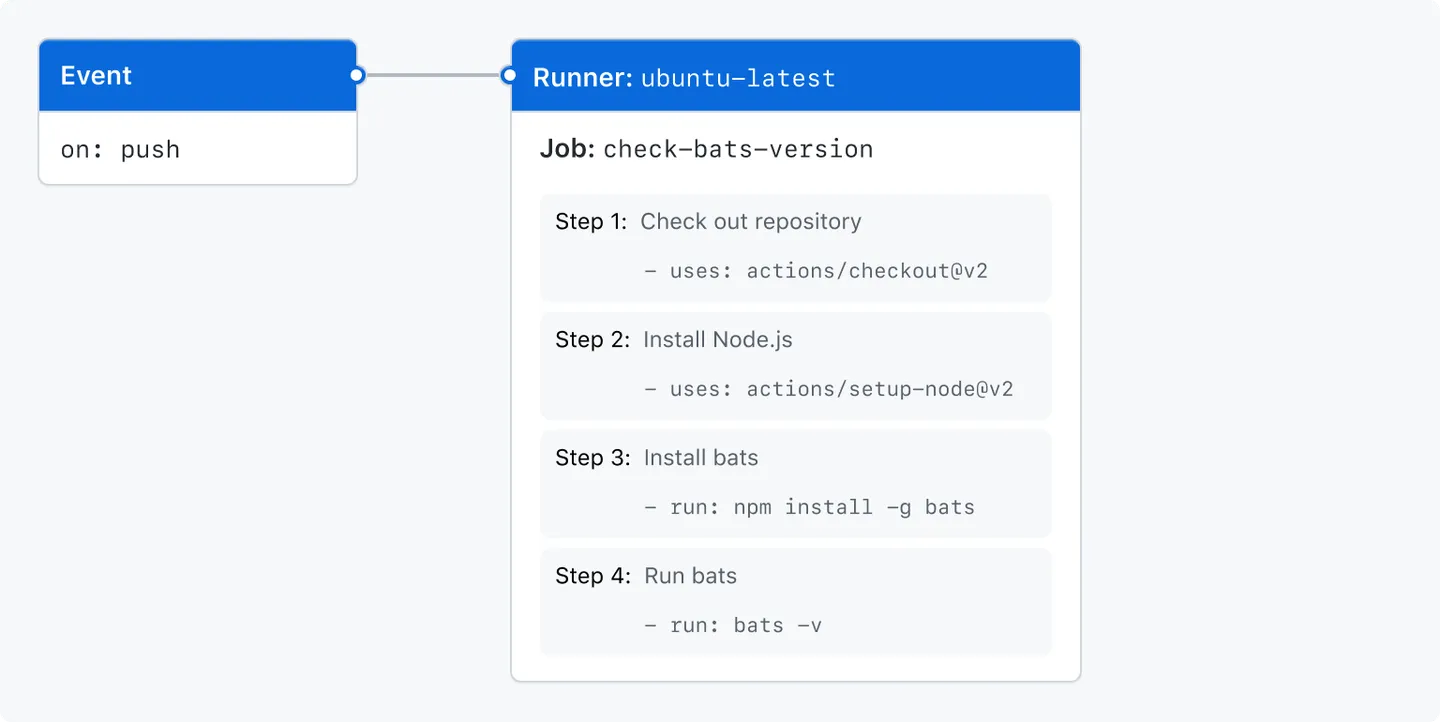
\includegraphics[width=0.95\textwidth]{figures/github/overview-actions-event.png}
          \caption{Egy workflow triggerét, runner-ét és feladatát bemutató ábra. A feladat 4 lépésre van bontva \cite{github}.}
           \label{overview-actions-event}
\end{figure}
%----------------------------------------------------------------------------
\chapter{\kli}
%----------------------------------------------------------------------------
\section{Tervezés}
A projekt tervezésekor kettő logikai részre osztottam a CLI-t. Front-end és back-end csomagokat külön fejlesztettem, melyeket végül egy projektbe integráltam be. A szándék az volt, hogy a back-end részt más által fejlesztett cli (avagy front-end) is tudja használni.
\section{Model-View-Controller ismertetése}
A MVC (Model-View-Controller) programtervezési mintát használtam a fejlesztéskor. Ez a modell segített abban, hogy külön válasszam a nézet réteget az adatrétegtől. A két réteg közötti kommunikációt egy vezérlői réteg oldja meg. Itt történik az adatok átadása, validálása az üzleti logika segítségével. Mivel a modulok a projetkben függetlenek egymástól köszönhetően az MVC alkalmazásának, így könnyű volt a későbbiekben változtatni és bővíteni az egyes modulok viselkedését. A tesztelhetőséget is nagyban megkönnyítette, mivel lehetőség adódott szimulálni (mock-olni) egy adott modult a másik modul tesztelésekor.

A hátrányait figyelembe vettem, amikor döntöttem a projektem felépítéséről. A legtöbb feladatot a back-end végzi el, a vezérlői réteg kódja pedig MVC boilerplate kód.
\section{Megvalósítás}
\subsection{Front-end}
Egy nyílt forráskodú könyvtárcsomag használatával felépítettem egy konzolos applikációt Go nyelv használatával. Az alkalmazás képes automatizáltan telepíteni és eltávolítani helm chart csomagokat a Kubernetes cluster-ből. Használata a következő flag-eken keresztül történik:
\begin{itemize}
    \item install, ahol az install után vár egy resource-t, amit telepít
    \item uninstall, ahol az uninstall után vár egy resource-t, amit eltávolít
\end{itemize}
Használati példák:
\begin{itemize}
    \item kli install --resource istio-operator
    \item kli uninstall --resource cluster-registry
\end{itemize}
Amikor meghívjuk az install flag-ek akkor a telepítés előtt ellenőrzés zajlik le, majd egy repository hozzáadás és frissítés. Ezután települ fel a helm csomag. A célja ennek a front-end csomagnak, hogy minimalizálja a függőségeit a külső moduloktól és csak a kubereflex back-end csomag funkcióira támaszkodjon.
\subsection{Back-end}
A kubereflex csomag felépítése modulárisra lett tervezve. A csomag fő modulja arra szolgál, hogy publikusan elérhetővé tegye az amúgy privát funkciókat az almodulokból. Emiatt a fő modul egyfajta kontroller szerepet tölt be. A külső modulok használata itt is minimalizálva van. Ideális esetben csak az almodulokat importálja be.
\subsubsection*{kubereflex modul}
Ez a back-end modul, melynek több almodulja van. Ebben a modulban található a üzleti logikai réteg, melynek segítségével történik meg az adatcsere.
\subsubsection*{kubectl almodul}
Ez az almodul felel az összes olyan funkcióért, amit a Kubernetes-ben kell végrehajtani. Ebben a csomagban van a névtér létrehozásához és már létrehozott névtér ellenőrzéséhez szükséges kódrészlet és majd itt lesz más csak kubernetes funkció is a jövőben, mely segít a cluster ellenőrzésében és a telepítési feltételek kialakításában, meglévő resource-ok konfigurálásában.
\subsubsection*{helm almodul}
Ez az almodul felel az összes olyan funkcióért, amit a Helm csomagkezelővel szeretnénk végrehajtani. Ilyen például az előre kész helm chart applikáció telepítése, törlése, repository hozzáadás, frissítés. Erre az almodulra fog a front-end nagyon sokat támaszkodni, mert az applikációk telepítése gyakran ezen az úton zajlik.
\subsubsection*{io almodul}
Ez az almodul felel minden fájl művelettel kapcsolatos funkciókért. Elsősorban a config fájlok betöltését teszi lehetővé a memóriába, de CRD leíró yaml fájl letöltésére is képes. Ennek az almodulnak a segítségével lehetséges a kontextus választó menü, mivel a kubernetes elérhető kontextusokat a konfigurációs fájlban vannak eltárolva.
\section{Tesztelés}
A csomagokhoz írtam teszt fájlokat, melyek minden egyes függvényt letesztelnek minta adatok segítségével. Ezek a tesztek sokat segítenek olyan hibák felderítésében, ami normális futtatáskor nem érzékelhető köszönhetően a teszt adatoknak.

A teszteléshez szükséges volt létrehoznom pár teszt specifikus függvényt, mely segít a teszt adatokat és a teszt klienseket beállítani, mielőtt a tesztelni kívánt függvény meghívásra kerülne.

\section{Kritikai elemzése}
A cli telepítési folyamatának reprezentálása lehetne felhasználóbarátabb azzal, hogy látszódna az elvégzett feladatok és az összes feladatok aránya, a várható idő amíg tart a telepítés és hiba esetén dokumentációt az adott hiba okáról.
Flag-ek kiosztása lehetne intuitívabb.
Tesztelés lehetne jobb.
\section{Továbbfejlesztési lehetőségek}
Ennek a CLI programnak a továbbfejlesztését úgy képzelem el, hogy olyan funkciók kerülnek implementálásra, melyek segítenek a felhasználónak az Istio operátor telepítésében.
\subsection{Operátor frissítése}
Meglévő klaszter telepítésnél lehetőség adódna frissíteni a komponenseket egy adott verziószámra. Ez a verziószám lehetne a legfrissebb kiadás, de régebbi verziók is rendelkezésre állnának.
\subsection{Log rendszer}
Lehetőség lenne megadni flag-eken keresztül, hogy milyen fájlba írja ki a kimenetet. Előre meg lehetne határozni több szintű log-olási részletességet és lehetőség adódna a standard output-ra való kiírás minimalizálására. A log fájl jól struktúrált lenne, ami segítené visszanézhetővé tenni a telepítési folyamat sikerességét. A log fájlban sokkal több részletet lehetne leírni az adott folyamatról vagy annak hibájáról, míg ez a részletesség a standard output-on zavaró lehetne. 
\subsection{Virtuálisgép integráció megvalósítása}
Lehetőség lenne a klaszterhez hozzáadni létező virtuálisgépeket, ezzel segítve a átmigrálást a klaszterre. Vannak olyan workload-ok, melyek jobban teljesítenek monolitikus applikációként és negatív hatással lenne a mikroszolgáltatási struktúra.
\subsection{Klaszterek létrehozása telepítés előtt}
A felhasználónak lehetősége lenne létrehozni előre definiált vagy a program alapértelmezett értékeit használva egy vagy több klasztert. Ennek megvalósítása minden cloud provider-nél más és más, mert az authetntikálás, authorizálás és API-n keresztüli parancsok egyediek.
\subsection{Automatizált post-install}
Miután megtörtént a telepítés és attach, lehetőség lenne kiválasztani a menüből előre összeállított vagy egyedileg definiált deploymenteket és helm chart-ok telepítésére. A post-install konfigurációs leíró fájlt meg lehetne adni egy flag-el, így teljesen automatikusan futna le a teljes folyamat. A felkínált post-install lista olyan elemeket tartalmazna, melyek nagy segítséget nyújthatnak a klaszter további üzemeltetésében. 
Előre üsszeállított deploymentekre példák:
\begin{itemize}
    \item Kubernetes dashboard
    \item Prometheus monitoring system
    \item Grafana dashboard
    \item cert-manager TLS cert manager
\end{itemize}



% Acknowledgements
%~~~~~~~~~~~~~~~~~~~~~~~~~~~~~~~~~~~~~~~~~~~~~~~~~~~~~~~~~~~~~~~~~~~~~~~~~~~~~~~~~~~~~~
%----------------------------------------------------------------------------
\chapter*{\koszonetnyilvanitas}\addcontentsline{toc}{chapter}{\koszonetnyilvanitas}
%----------------------------------------------------------------------------

Ez nem kötelező, akár törölhető is. Ha a szerző szükségét érzi, itt lehet köszönetet nyilvánítani azoknak, akik hozzájárultak munkájukkal ahhoz, hogy a hallgató a szakdolgozatban vagy diplomamunkában leírt feladatokat sikeresen elvégezze. A konzulensnek való köszönetnyilvánítás sem kötelező, a konzulensnek hivatalosan is dolga, hogy a hallgatót konzultálja.


% List of Figures, Tables
%~~~~~~~~~~~~~~~~~~~~~~~~~~~~~~~~~~~~~~~~~~~~~~~~~~~~~~~~~~~~~~~~~~~~~~~~~~~~~~~~~~~~~~
%\listoffigures\addcontentsline{toc}{chapter}{\listfigurename}
%\listoftables\addcontentsline{toc}{chapter}{\listtablename}


% Bibliography
%~~~~~~~~~~~~~~~~~~~~~~~~~~~~~~~~~~~~~~~~~~~~~~~~~~~~~~~~~~~~~~~~~~~~~~~~~~~~~~~~~~~~~~
\addcontentsline{toc}{chapter}{\bibname}
\bibliography{bib/mybib}


% Appendix
%~~~~~~~~~~~~~~~~~~~~~~~~~~~~~~~~~~~~~~~~~~~~~~~~~~~~~~~~~~~~~~~~~~~~~~~~~~~~~~~~~~~~~~
%----------------------------------------------------------------------------
\appendix
%----------------------------------------------------------------------------
\chapter*{\fuggelek}\addcontentsline{toc}{chapter}{\fuggelek}
\setcounter{chapter}{\appendixnumber}
%\setcounter{equation}{0} % a fofejezet-szamlalo az angol ABC 6. betuje (F) lesz
\numberwithin{equation}{section}
\numberwithin{figure}{section}
\numberwithin{lstlisting}{section}
%\numberwithin{tabular}{section}

%----------------------------------------------------------------------------
\section{A TeXstudio felülete}
%----------------------------------------------------------------------------
\begin{figure}[!ht]
\centering
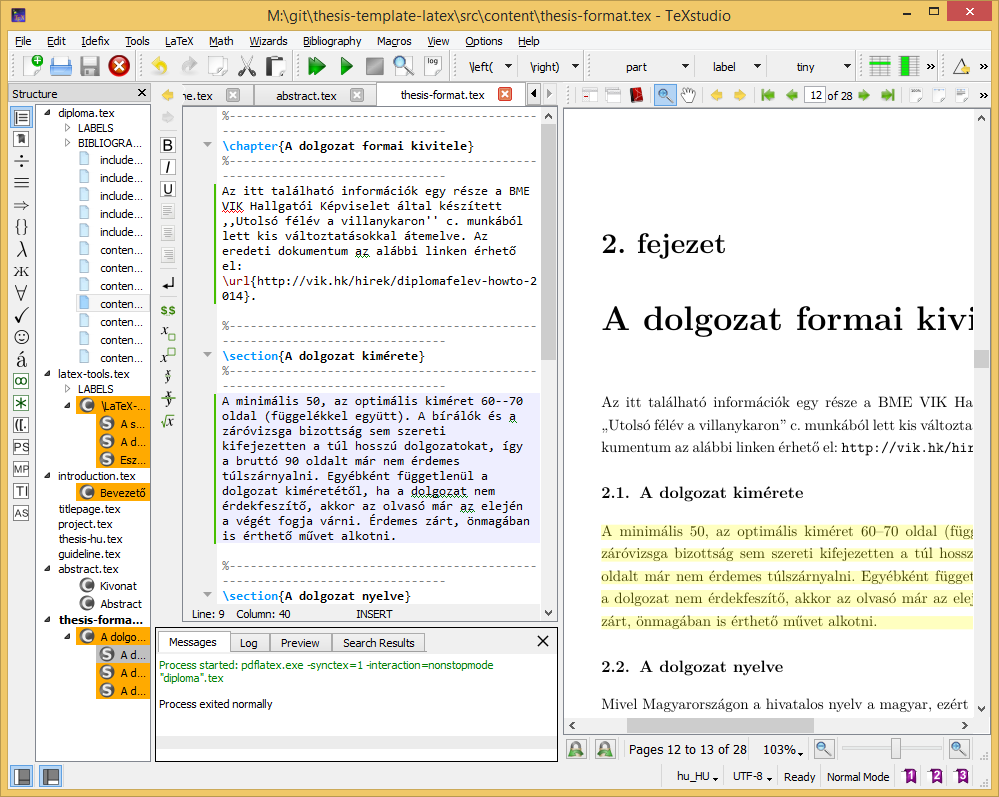
\includegraphics[width=150mm, keepaspectratio]{figures/TeXstudio.png}
\caption{A TeXstudio \LaTeX-szerkesztő.} 
\end{figure}

%----------------------------------------------------------------------------
\clearpage\section{Válasz az ,,Élet, a világmindenség, meg minden'' kérdésére}
%----------------------------------------------------------------------------
A Pitagorasz-tételből levezetve
\begin{align}
c^2=a^2+b^2=42.
\end{align}
A Faraday-indukciós törvényből levezetve
\begin{align}
\rot E=-\frac{dB}{dt}\hspace{1cm}\longrightarrow \hspace{1cm}
U_i=\oint\limits_\mathbf{L}{\mathbf{E}\mathbf{dl}}=-\frac{d}{dt}\int\limits_A{\mathbf{B}\mathbf{da}}=42.
\end{align}


%\label{page:last}
\end{document}
